% -*- TeX:UK -*-
\chapter{Descriptive statistics}
\begin{refsection}

\abstract{Descriptive statistics summarizes data vectors by parameters of position, dispersion, shape and concentration. This can be done assuming the data follow a given distribution (most commonly \Name{Gauss}' normal distribution), or it can be done parameter-free. }

Good introductions to elementary statistics are \parencite{Kre-79, Fre-65}.

The \textbf{breakdown point} of a statistics is the number of data that can be replaced with arbitrary values before a measure can collapse to zero or explode to infinity. The arithmetic mean, for example, has a breakdown point of zero, because a single \( \AbsVec{x}_i = \infty\ \rightarrow\ \bar{\AbsVec{x}} = \infty \). Similarly, for any \( \AbsVec{x}_i = 0\ \rightarrow\ \check{\AbsVec{x}} = 0, \tilde{\AbsVec{x}} = 0 \). For the median, the breakdown point is \SI{50}{\%}. This is the highest value possible, because with higher contamination it would no longer be possible to distinguish the distribution of the data from the distribution of the contamination. If the \skalar{y}\si{\%} highest and lowest values are trimmed (removed) from the data, the breakdown point of the trimmed arithmetic mean becomes \skalar{y}\si{\%}.

The \textbf{influence function} describes how a measure is affected by changing (or removing) a single data point (empirical influence function) or by a slight change in the distribution of the data. Ideally, the influence function should be bounded and differentiable (without discontinuities).

The \textbf{efficiency} of a parameter or procedure measures how many data points are required to achieve a given purpose. The \textbf{relative efficiency} compares the efficiency of two procedures by dividing the number of data required by one of them by the number of data required by the procedure considered the ``best possible''. Because the efficiency of some procedures depends on sample size, the \textbf{asymptotic relative efficiency} measures the relative efficiency as the sample size grows toward infinity.

The unit \texttt{descript} has the following interface
\begin{lstlisting}[caption=Interface of descript]
UNIT Deskript;

{ descriptive statistics on vectors and matrices }

INTERFACE

USES Math, mathfunc, Vector, Matrix;

CONST
  DeskriptError: BOOLEAN = FALSE;

{ ************************** Position ******************************* }

FUNCTION ArithmeticMean(Data: VectorTyp): float;

FUNCTION GeometricMean(Data: VectorTyp): float;

FUNCTION HarmonicMean(Data: VectorTyp): float;

FUNCTION GeneralMean(Data, Gewichte: VectorTyp; Exponent: float): float;

{ ********************************** Scale ****************************** }

FUNCTION Gini(Data: VectorTyp; Mean: float): float;

FUNCTION Covariance(CONST X, Y: VectorTyp): float;

FUNCTION MeanDeviationFromMean(Data: VectorTyp): float;

FUNCTION MedianDeviationFromMean(Data: VectorTyp): float;

FUNCTION Variance(Data: VectorTyp): float;

FUNCTION StandardDeviation(VAR Data: VectorTyp): double;

FUNCTION CoefficientOfVariation(Mean, v: float; n: WORD): float;

{ ***************************** Moments *********************************** }

FUNCTION Mue(CONST Data: VectorTyp; Mean: float; k: WORD): float;

FUNCTION Skewness(CONST Data: VectorTyp; Mean, StaDev: float): float;

FUNCTION ExcessKurtosis(CONST Data: VectorTyp; Mean, StaDev: float): float;

{ ***************************** Grouped data ************************ }

FUNCTION WeightedMean(Means, Vars, Lengths: VectorTyp): float;

FUNCTION WeightedStandardDeviation(Means, Vars, Lengths: VectorTyp): float;

{ ***************************** Concentration *************************** }

FUNCTION LorenzMuenzner(Data: VectorTyp; VAR xVektor, yVektor: VectorTyp): float;

FUNCTION HerfindahlIndex(Data: VectorTyp): float;

{ *********************** non-parametric position ************************* }

FUNCTION HiMed(CONST SortedData: VectorTyp): float;

FUNCTION LoMed(CONST SortedData: VectorTyp): float;

FUNCTION Median(VAR Data: VectorTyp): float;

FUNCTION WeightedHiMed(CONST SortedData: MatrixTyp): float;

FUNCTION WeightedLoMed(CONST SortedData: MatrixTyp): float;

FUNCTION WeightedMedian(VAR Data: MatrixTyp): float;

FUNCTION Quantile(VAR Data: VectorTyp; q: float): float;

FUNCTION TriMedian(Data: VectorTyp): float;

FUNCTION HodgesLehmann(Data: VectorTyp): float;

FUNCTION NaiveHodgesLehmann(Data: VectorTyp): float;

{ *********************** non-parametric scale ************************* }

FUNCTION InterQuantilDistance(Q1, Q3: float): float;

FUNCTION MAD(Data: VectorTyp): double;

FUNCTION StandardErrorOfMedian(Data: VectorTyp): float;

FUNCTION QuantileDispersionCoefficient(Q1, Q3: float): float;

FUNCTION Sn(VAR Data: VectorTyp): float;

FUNCTION NaiveSn(VAR Data: VectorTyp): float;

FUNCTION Qn(VAR Data: VectorTyp): float;

FUNCTION NaiveQn(VAR Data: VectorTyp): float;

{ *********************** non-parametric moments ************************* }

FUNCTION Ell2(CONST SortedData: VectorTyp): float;

FUNCTION Ell3(CONST SortedData: VectorTyp): float;

FUNCTION Ell4(CONST SortedData: VectorTyp): float;

FUNCTION QuartileCoefficientOfSkewness(Q1, Q2, Q3: float): float;

FUNCTION CentilCoeffKurtosis(Data: VectorTyp): float;

{ ******************** Standardise and normalise vector ****************** }

PROCEDURE MeanNormalise(VAR Data: VectorTyp);
{ subtract arithmetic mean from all elements }

PROCEDURE Z_Standardise(VAR Data: VectorTyp);
{ subtract mean and divide by standard deviation }

PROCEDURE RobustStandardise(VAR Data: VectorTyp);
{ subtract median and divide by Qn }

{ ************************ Description of matrices *********************** }

PROCEDURE VarCovarMatrix(CONST Data: MatrixTyp; VAR VarCovar: MatrixTyp);

PROCEDURE VarCov(CONST Data: MatrixTyp; VAR VarCovar: MatrixTyp);

PROCEDURE MeanVector(CONST Data: MatrixTyp; VAR Mean: VectorTyp);

PROCEDURE StaVector(CONST Data: MatrixTyp; VAR Sta: VectorTyp);

{ ***************** Standardise and normalise matrix columns *************** }

PROCEDURE CentreMatrix(VAR A: MatrixTyp);

PROCEDURE StandardiseMatrix(VAR A: MatrixTyp);

PROCEDURE RobustStandardiseMatrix(VAR A: MatrixTyp);

{ *********************** Distances and outliers *********************** }

PROCEDURE MahalanobisDistance(CONST Data: MatrixTyp; VAR Dm: VectorTyp);

PROCEDURE RobustDistance(CONST Data: MatrixTyp; VAR Dr: VectorTyp);


IMPLEMENTATION

VAR
  CH: CHAR;
\end{lstlisting}

\section{Normally distributed data}

\subsection{Position}

If we have a vector of data, we may want to characterise them by giving a value that is ``typical'' for all of them, in the sense that if we did not have a particular value, we could use this typical value as an estimate without too much error. This typical value is called position. The position of a data vector is given by its mean.
The most commonly used mean is the arithmetic mean
\begin{equation}
  \bar{\AbsVec{x}} = \frac{\sum_{i=1}^n{\AbsVec{x}_i}}{n}
\end{equation}
For normally distributed data, the arithmetic mean is the maximum likelihood estimator for missing values, which is one reason for its popularity. In other words, for the arithmetic mean \( \sum_{i=1}^n{(\AbsVec{x}_i - \bar{\AbsVec{x}})} = 0 \) and \( \sum_{i=1}^n{(\AbsVec{x}_i - \bar{\AbsVec{x}})}^2 \) is minimal.

When calculating the sum over all elements, we use the \Name{Neumaier}-sum to prevent catastrophic loss of precision if the data are of very different magnitude. Because the function \texttt{NeumaierSum} ignores NaN, we have to use the function \texttt{ActualElements} rather than \texttt{VectorLength} for the denominator:

\begin{lstlisting}[caption=arithmetic mean]
  FUNCTION ArithmeticMean(Data: VectorTyp): float;

  VAR
    i: WORD;

  BEGIN
    i := VectorLength(Data);
    IF i > 0
      THEN
        Result := NeumaierSum(Data) / ActualElements(Data)
      ELSE
        BEGIN
          ch := WriteErrorMessage('Arithmetic mean from vector of length 0');
          DeskriptError := TRUE;
        END;
  END;
\end{lstlisting}

The geometric mean is defined as
\begin{equation}
  \check{\AbsVec{x}} = \sqrt[n]{\prod_{i=1}^n{\AbsVec{x}_i}} =  \exp\left(\frac{1}{n} \sum_{i=1}^n{\ln(\AbsVec{x}_i)} \right)\ \forall\ \AbsVec{x}_i > 0
\end{equation}
If at least one of the \skalar{\AbsVec{x}_i} is zero, the geometric mean becomes zero. Compared to the arithmetic mean, \( \check{\AbsVec{x}} \leq \bar{\AbsVec{x}} \). The logarithm of the geometric mean is the arithmetic mean of the logarithms of the data, the geometric mean is the length of the sides of a hypercube that has the same volume as the hyper-brick with the side-lengths \skalar{\AbsVec{x}_i}. For implementation in a computer, the logarithmic form of the algorithm is preferred, as it is less likely to produce over- or under-flows. Even if the order of magnitude of the data were vastly different (in which case an average wouldn't make sense), the order of the logarithms is comparable. Therefore the use of a \Name{Neumaier}-sum is not required.

\begin{lstlisting}[caption=Geometric mean]
  FUNCTION GeometricMean(Data: VectorTyp): float;

  VAR
    Sum, x: float;
    n, i: WORD;

  BEGIN
    n := VectorLength(Data);
    IF (n = 0)
      THEN
        BEGIN
          ch := WriteErrorMessage('Geometric mean from vector of length 0');
          DeskriptError := TRUE;
          EXIT;
        END;
    CASE VectorSignum(Data) OF
      -1: BEGIN
            ch := WriteErrorMessage('Geometric mean from negative data');
            DeskriptError := TRUE;
            EXIT;
          end;
      0: Result := 0;  // product IS 0 if any of the factors is 0
      1: BEGIN
           n := 0;
           Sum := 0;
           FOR i := 1 TO VectorLength(Data) DO
             BEGIN
               x := GetVectorElement(Data, i);
               IF IsNaN(x)
                 THEN
                 ELSE
                   BEGIN
                     INC(n);
                     Sum := Sum + Ln(x);
                   END;
               Result := Exp(Sum / n);
             END;
         END;
    END; { case }
  END;
\end{lstlisting}

The harmonic mean is defined as
\begin{equation}
  \tilde{\AbsVec{x}} = \frac{n}{\sum_{i=1}^n{\AbsVec{x}_i^{-1}}} \ \forall\ \AbsVec{x}_i > 0
\end{equation}
The reciprocal of the harmonic mean is the arithmetic mean of the reciprocals of the data. If at least on of the \skalar{\AbsVec{x}_i} is zero, the harmonic mean is defined as zero because \( \lim_{\AbsVec{x}_i \rightarrow 0}  \tilde{\AbsVec{x}} = 0 \). The harmonic mean is smaller or equal than the geometric mean.

\begin{lstlisting}[caption=Harmonic mean]
  FUNCTION HarmonicMean(Data: VectorTyp): float;

  VAR
    Sum, x: float;
    i, j, n: WORD;

  BEGIN
    n := VectorLength(Data);
    IF (n = 0)
      THEN
        BEGIN
          CH := WriteErrorMessage('Harmonic mean from vector of length 0');
          DeskriptError := TRUE;
          EXIT;
        END;
    CASE VectorSignum(Data) OF
      -1: BEGIN
            WriteErrorMessage('Harmonic mean from negative data');
            DeskriptError := TRUE;
            EXIT;
          end;
       0: Result := 0;
       1: BEGIN
            Sum := 0;
            j := 0;
            n := VectorLength(Data);
            FOR i := 1 TO n DO
              BEGIN
                x := GetVectorElement(Data, i);
                IF IsNaN(x)
                  THEN // ignore
                  ELSE
                    BEGIN
                      Sum := Sum + 1 / x;
                      INC(j);
                    END;
              END;
            Result := j / Sum;
          END;
    END; // CASE
  END;
\end{lstlisting}

\begin{figure}
 \caption{Geometric interpretation of the various means of two data, \skalar{a} and \skalar{b}. }
 \label{fig:GeoMean}
 \centering
 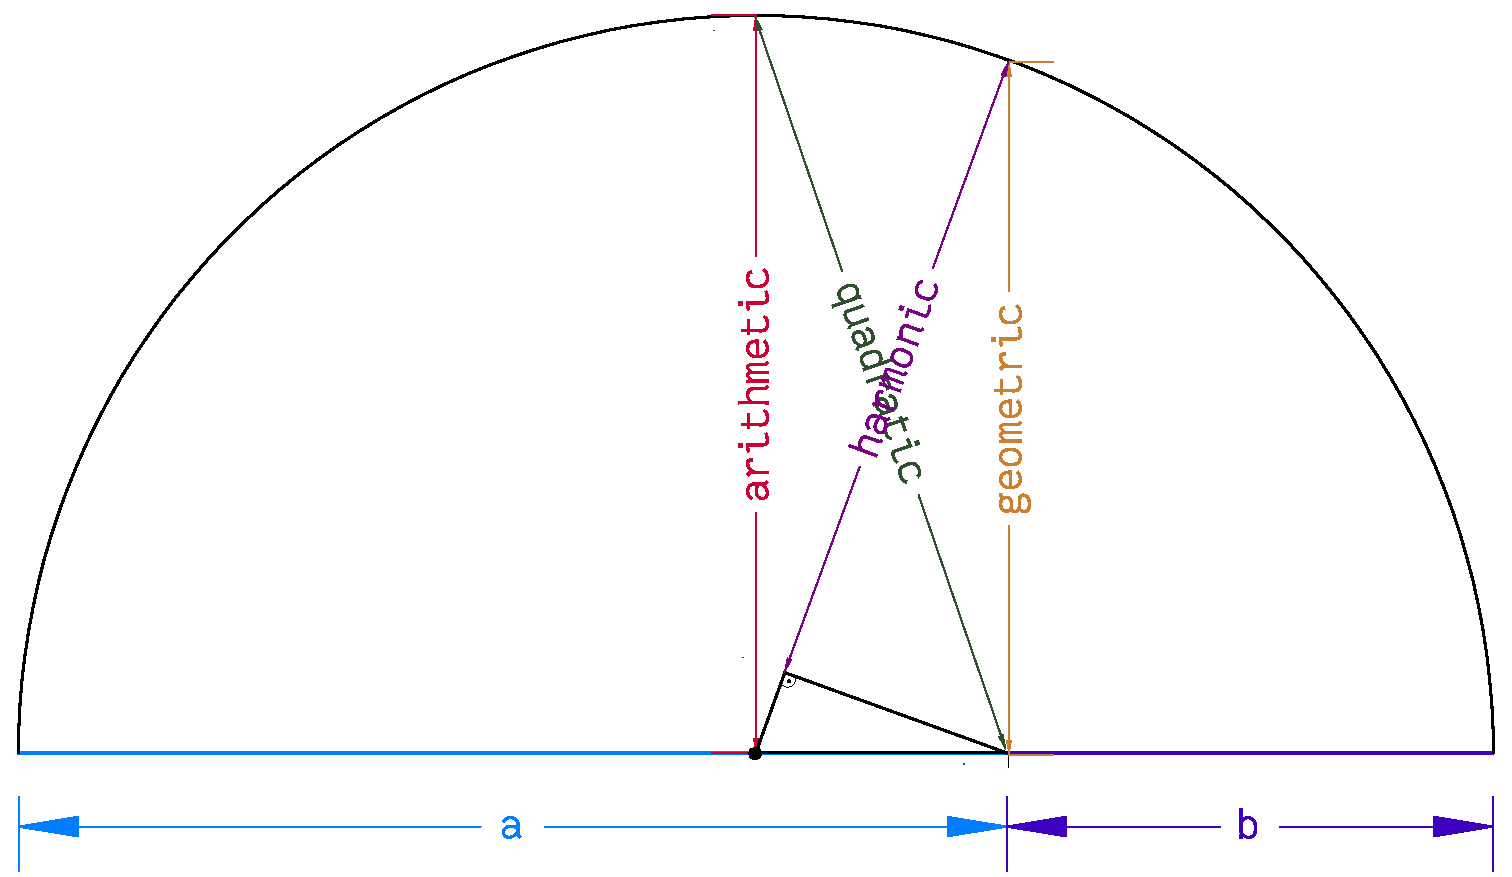
\includegraphics[width=0.75\textwidth]{Graphics/GeometricInterpretationMean}
\end{figure}

The quadratic mean (\Name{Euklid}ian mean, root mean square RMS) is defined as
\begin{equation}
  \mathrm{RMS} = \sqrt[2]{\frac{\sum_{i=1}^n{\AbsVec{x}_i^2}}{n}}
\end{equation}
The cubic mean is defined analogously. The RMS is technically important to calculate the effective voltage and current in alternating power.

The weighted \Name{Hölder}\index{Hölder@\textsc{Hölder, Ludwig Otto} 1859--1937!mean} (general) mean is defined for \( \AbsVec{x}_i \in \mathbb{R} \geq 0 \), a whole number \(z \neq 0 \) and a weight vector \AbsVec{w} with \( \sum_{i=1}^n{w_i} = 1\)
\begin{equation}
  M_\AbsVec{w}^z(\AbsVec{x}) = \sqrt[z]{\sum_{i=1}^n{\AbsVec{w}\AbsVec{x}^z_i}}
\end{equation}
where in the unweighted case all \( \AbsVec{w}_i = 1/n \). Depending on the choice of \skalar{z} we get different means:
\begin{description}
  \item[\( \lim_{z \rightarrow -\infty} \)]{minimum \( M^{-\infty}(\AbsVec{x}) = \min(\AbsVec{x}_i)  \)}
  \item[\( z = -1 \)]{harmonic mean \( M^{-1}(\AbsVec{x}) = \frac{n}{\sum_{i=1}^n{\AbsVec{x}_i^{-1}}}  \)}
  \item[\( \lim_{z \rightarrow 0} \)]{geometric mean  \( M^{0}(\AbsVec{x}) = \sqrt[n]{\prod_{i=1}^n{\AbsVec{x}_i}}  \)}
  \item[\( z = 1 \)]{arithmetic mean  \( M^1(\AbsVec{x}) = \frac{\sum_{i=1}^n{\AbsVec{x}_i}}{n}  \)}
  \item[\( z = 2 \)]{quadratic mean  \( M^2(\AbsVec{x}) = \sqrt[2]{\frac{\sum_{i=1}^n{\AbsVec{x}_i^2}}{n}}  \)}
  \item[\( z = 3 \)]{cubic mean \( M^3(\AbsVec{x}) = \sqrt[3]{\frac{\sum_{i=1}^n{\AbsVec{x}_i^3}}{n}}  \)}
  \item[\ldots]{}
  \item[\( \lim_{z \rightarrow \infty} \)]{maximum \( M^{\infty}(\AbsVec{x}) = \max(\AbsVec{x}_i)  \)}
\end{description}

\begin{lstlisting}[caption=\Name{Hölder} mean]
  FUNCTION GeneralMean(Data, Gewichte: VectorTyp; Exponent: float): float;

  VAR
    i, n: WORD;
    Sum: float;

  BEGIN
    Sum := 0;
    n := VectorLength(Data);
    IF (n = 0)
      THEN
        BEGIN
          CH := WriteErrorMessage('General mean from vector of length 0');
          DeskriptError := TRUE;
          EXIT;
        END;
    IF (n <> VectorLength(Gewichte))
      THEN
        BEGIN
          CH := WriteErrorMessage( 'General mean: unequal vector lengths of data and weights');
          DeskriptError := TRUE;
          EXIT;
        END;
    FOR i := 1 TO n DO
      Sum := Sum + GetVectorElement(Gewichte, i) * pot(GetVectorElement(Data, i), Exponent);
    Result := pot(Sum, 1 / Exponent);
  END;
\end{lstlisting}

The \textbf{f-mean} is a generalisation of the \Name{Hölder}-mean
\begin{equation}
  M_\AbsVec{w}^f = f^{-1} \left( \sum_{i=1}^n{\AbsVec{w}_i f(\AbsVec{x}_i)} \right)
\end{equation}
where in case of the \Name{Hölder}-mean \( f(\AbsVec{x}) = \AbsVec{x}^z \). For example, if \AbsVec{x} contains the returns of a capital from year 1 to \skalar{n}, then the f-mean with \( f(\AbsVec{x}) = \ln(\AbsVec{x} + 1) \) is the average return.

\subsection{Dispersion}

As discussed above, we can describe a data vector by a parameter of location, that is, a mean. However, in addition to the location, we also would like information about how much the data spread around that mean, \Foreign{i.e.}, how much error are we likely to make, if we use the mean to fill in a missing value. This is measured by parameters of dispersion.

\subsubsection{Variance and Covariance}

The covariance of two data vectors \AbsVec{X, Y} is defined as
\begin{equation}
  s_\AbsVec{x,y}^2 = 1/n \sum_{i=1}^n{(\AbsVec{x}_i - \bar{\AbsVec{x}}) (\AbsVec{y}_i - \bar{\AbsVec{y}})}
\end{equation}
The variance of a vector is the covariance with itself, \texttt{Covariance(\AbsVec{x,x})}.

To perform this calculation, two loops over the data are required, once to calculate the averages and once to calculate the variance. Here we use an alternative way that calculates both in a single loop:
\begin{align}
  s^2_1              & = 0.0  \\
  \bar{\AbsVec{x}}_1 & = \AbsVec{x}_1 \notag \\
  \bar{\AbsVec{y}}_1 & = \AbsVec{y}_1 \notag \\
  s^2_i              & = s_{i-1} \times \frac{i-2}{i-1} + \frac{(\AbsVec{x}_i - \bar{\AbsVec{x}}_{i-1})(\AbsVec{y}_i - \bar{\AbsVec{y}}_{i-1})}{i},\quad i = 2\ldots n \notag \\
  \bar{\AbsVec{x}}_i & = \bar{\AbsVec{x}}_{i-1} + \frac{\AbsVec{x}_i - \bar{\AbsVec{x}}_{i-1}}{i} \notag \\
  \bar{\AbsVec{y}}_i & = \bar{\AbsVec{y}}_{i-1} + \frac{\AbsVec{y}_i - \bar{\AbsVec{y}}_{i-1}}{i} \notag
\end{align}

\begin{lstlisting}[caption=Covariance of two vectors]
  FUNCTION Covariance(CONST X, Y: VectorTyp): float;

  VAR
    n, Count, i, j: WORD;
    CH: CHAR;
    xi, yi, xAv, yAv, s: float;

  BEGIN
    n := VectorLength(X);
    IF (n = 0)
      THEN
        BEGIN
          CH := WriteErrorMessage('Covariance from vector of length 0');
          DeskriptError := TRUE;
          EXIT;
        END;
    IF (n <> VectorLength(Y))
      THEN
        BEGIN
          CH := WriteErrorMessage('Covariance of vectors of unequal length ');
          DeskriptError := TRUE;
          EXIT;
        END;
    j := 0;
    REPEAT                            // find first complete pair OF data
      INC(j);
      xi := GetVectorElement(X, j);
      yi := GetVectorElement(Y, j);
    UNTIL NOT (IsNaN(xi) OR IsNaN(yi));
    xAv := xi;
    yAv := yi;
    s := 0.0;
    Count := 1;
    FOR i := Succ(j) TO n DO
      BEGIN
        xi := GetVectorElement(X, i);
        yi := GetVectorElement(Y, i);
        IF (IsNan(xi) OR IsNaN(yi))
          THEN
          ELSE
            BEGIN
              INC(Count);
              s := s * ((Count - 2) / (Count - 1)) + (xi - xAv) * (yi - yAv) / Count;
              xAv := xAv + (xi - xAv) / Count;
              yAv := yAv + (yi - yAv) / Count;
            END;
      END;
    Result := s;
  END;


  FUNCTION Variance(Data: VectorTyp): float;

  BEGIN
    Result := Covariance(Data, Data);
  END;
\end{lstlisting}

The standard deviation \skalar{\sigma} of a data vector is the square root of its variance. It has the same unit as the mean, which makes them comparable. If the data are normally distributed,   \SI{68.3}{\%} of the data will be within the range \( \pm \sigma \), \SI{95.4}{\%} within \( \pm 2\sigma \) and \SI{99.7}{\%} within \( \pm 3\sigma \).
\begin{lstlisting}
   function StandardDeviation(var Data: VectorTyp): float;

   begin
     Result := sqrt(Covariance(Data, Data));
   end;
\end{lstlisting}

The standard error of the mean is \( \sigma_{\bar{\AbsVec{x}}} =  \frac{\sqrt{\sigma^2}}{\sqrt{n}} \), thus, increasing \skalar{n} will decrease this error, but with diminishing return.
\begin{lstlisting}
  FUNCTION StandardErrorOfMean(v: float; n: WORD): float;

  BEGIN
    IF n > 0
      THEN
        StandardErrorOfMean := Sqrt(v) / Sqrt(n)
      ELSE
        BEGIN
          WriteErrorMessage(' Standard error of mean for n = 0');
          DeskriptError := TRUE;
        END;
  END;
\end{lstlisting}



The coefficient of variation (unitised risk) is the standard deviation divided by the absolute value of the mean: \( \mathrm{CV} = \frac{\sqrt{\sigma^2}}{|\mu|} \), often multiplied with \SI{100}{\%}. It is used to express the precision of an assay. As a number without unit it is independent of the unit in which the data were measured. Warning: If the data are not measured on a rational scale, the mean may be zero (\Foreign{e.g.}, temperatures on the \si{\celsius} scale near freezing) and the CV is affected by small fluctuations of the mean.
\begin{lstlisting}
  FUNCTION CoefficientOfVariation(Mean, v: float; n: WORD): float;

  BEGIN
    IF Abs(mean) > Zero
      THEN
        Result := Sqrt(v) / Abs(Mean)
      ELSE
        BEGIN
          WriteErrorMessage(' Coefficient of variation with mean 0');
          DeskriptError := TRUE;
        end;
  END;
\end{lstlisting}

\subsubsection{Other measures of dispersion}

Alternatively, on can calculate the distance of all data points from the mean, and then determine the mean or median of those:
\begin{lstlisting}
  FUNCTION MeanDeviationFromMean(Data: VectorTyp): float;

  VAR
    Mean, Sum: float;
    i, j, n: WORD;

  BEGIN
    n := VectorLength(Data);
    IF (n = 0)
      THEN
        BEGIN
          CH := WriteErrorMessage('Mean deviation of mean from vector of length 0');
          DeskriptError := TRUE;
          EXIT;
        END;
    Mean := ArithmeticMean(Data);
    Sum := 0;
    FOR i := 1 TO n DO
      Sum := Sum + Abs(Mean - GetVectorElement(Data, i));
    Result := Sum / n;
  END;


  FUNCTION MedianDeviationFromMean(Data: VectorTyp): float;

  VAR
    Mean: float;
    Abweichungen: VectorTyp;
    i: WORD;

  BEGIN
    CreateVector(Abweichungen, VectorLength(Data), 0.0);
    Mean := ArithmeticMean(Data);
    CreateVector(Abweichungen, VectorLength(Data), 0.0);
    FOR i := 1 TO VectorLength(Data) DO
      SetVectorElement(Abweichungen, i, Abs(Mean - GetVectorElement(Data, i)));
    ShellSort(Abweichungen);
    MedianDeviationFromMean := Median(Abweichungen);
    DestroyVector(Abweichungen);
  END;
\end{lstlisting}

\subsection{\Name{Pearson} moments}

Moments describe the shape of a distribution curve. The 0th moment is the total probability, that is, the integral of the distribution curve and hence always unity. The 1st moment is the expected value, that is, the mean. The 2nd moment is the variance. The 3rd moment is the skewness (lopsidedness, asymmetry), the 4th moment the kurtosis (heaviness of the tail). Higher moments can be defined, but are not commonly used. The moment is calculated from
\begin{equation}
  \mu_k = \frac{1}{n} \sum_{i=1}^n{(\AbsVec{x}_i-\bar{\AbsVec{x}})^k}
\end{equation}
They are then standardised by dividing them by \skalar{\sigma^k}.

\begin{lstlisting}
  FUNCTION Mue(CONST Data: VectorTyp; Mean: float; k: WORD): float;

  VAR
    Sum: float;
    i, n: WORD;

  BEGIN
    Sum := 0;
    n := VectorLength(Data);
    IF (n = 0)
      THEN
        BEGIN
          CH := WriteErrorMessage('Mue from vector of length 0');
          DeskriptError := TRUE;
          EXIT;
        END;
    FOR i := 1 TO n DO
      Sum := Sum + pot(GetVectorElement(Data, i) - Mean, k);
    Result := Sum / n;
  END;
\end{lstlisting}

Skewness, \( \mu_3/\sigma^3\), is a measure of asymmetry of a distribution, and can be
\begin{description}
  \item[negative]{tail is on the left side, left-skewed = right-leaning}
  \item[zero]{the tails balance, but the distribution is not necessarily symmetrical}
  \item[positive]{tail is on the right side, right-skewed = left-leaning}
\end{description}
, at least for simple unimodal distributions.

\begin{lstlisting}
  FUNCTION Skewness(CONST Data: VectorTyp; Mean, StaDev: float): float;

  BEGIN
    Result := Mue(Data, Mean, 3) / pot(StaDev, 3);
  END;
\end{lstlisting}

Alternative measures of skewness have been suggested by \Name{Pearson}:
\begin{equation}
  \frac{\bar{\AbsVec{x}} - \mathrm{mode}(\AbsVec{x})}{\sigma},\ \frac{3 \bar{\AbsVec{x}} - \breve{\AbsVec{x}}}{\sigma}
\end{equation}

The kurtosis (from Gr. curved, arching) is the 4th standardised \Name{Pearson} moment \( \mu_4/\sigma^4\). Data within one standard deviation of the mean contribute little to its value, because raising the \skalar{z}-standardised datum to the 4th power will make them close to zero. Only data away from the peak -- that is, outliers -- contribute to the kurtosis. The kurtosis parameter is a measure of the combined weight of the tails, relative to the centre of the distribution. The normal distribution has a kurtosis of \num{3}. Thus, we get the \textbf{excess kurtosis} by subtracting \num{3} from the moment. The result can be
\begin{description}
  \item[negative]{, then the distribution is called platykurtic and has fewer and less extreme outliers }
  \item[zero]{, then the distribution is called mesokurtic and has about as many outliers}
  \item[positive]{, then the distribution is called leptokurtic and has more, and more extreme outliers}
\end{description}
than the normal distribution.

\begin{lstlisting}
  FUNCTION ExcessKurtosis(CONST Data: VectorTyp; Mean, StaDev: float): float;

  BEGIN
    Result := (Mue(Data, Mean, 4) / pot(StaDev, 4)) - 3.0;
  END;
\end{lstlisting}

\subsection{Concentration}

\subsubsection{\Name{Lorenz-Münzner}-curve and \Name{Gini}-coefficient}

\begin{figure}
 \caption{\Name{Lorenz-Münzner}-plot. For details see text. }
 \label{fig:Lorenz}
 \centering
 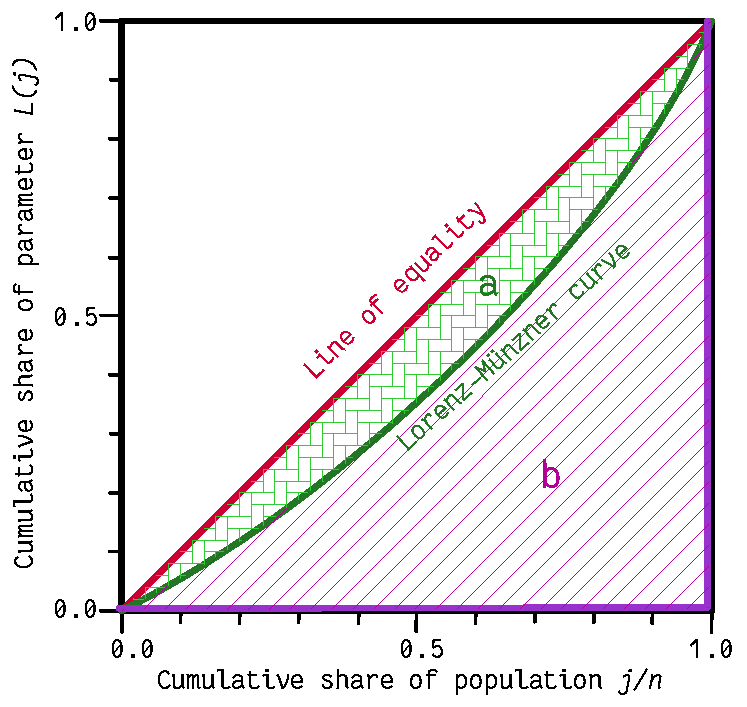
\includegraphics[width=0.75\textwidth]{Graphics/Lorenz-Munzner}
\end{figure}

The \Name{Lorenz-Münzner} curve of an data vector \AbsVec{x} sorted in non-decreasing order (see fig. \ref{fig:Lorenz}) is given by
\begin{equation}
  L(j) = \sum_{i=1}^j{\frac{\AbsVec{x}_i}{n\mu}} = \sum_{i=1}^j{\AbsVec{l}_j}
\end{equation}
and is the cumulative fraction of the data for every position \skalar{j}. If \( \AbsVec{x}_i = \mu\ \forall\ i \) (all data are the same), then a plot of \skalar{L(j)} vs \skalar{j/n} is a straight line through the origin with slope  one (line of equality, \emph{red}). In the other extreme, if all \skalar{\AbsVec{x}_i} except one are zero, then the \Name{Lorenz-Münzner} curve consist of two straight lines (\emph{purple}), one from (0, 0) to (1, 0) and the second perpendicular to (1, 1) . Together with the line of equality, they form a triangle with area \num{0.5}.

Real data will form a curve between those extremes, and the \Name{Gini}-coefficient \parencite{Gin-36} is the area between this curve and the line of equality, divided by the area of the triangle: \( G = a/(a + b) \), because \( a + b = 0.5 \), this is equal to \( G = 2a \). If \( \AbsVec{x}_i \geq 0\ \forall\ i \), the \Name{Gini}-coefficient ranges from \( 0\ldots 1 \). If the parameter is distributed equally, and all data are on the line of equality, the \Name{Gini}-coefficient is zero, in case of maximal inequality it becomes \num{1}. Thus
\begin{equation}
   G = 2 a = \sum_{i=1}^n{\AbsVec{l}_i \left( \frac{i-1}{n} + \frac{i}{n} \right)} - \frac{1}{2} = \sum_{i=1}^n{\AbsVec{l}_i \frac{2i - n - 1}{2n}}
\end{equation}

\begin{lstlisting}
  FUNCTION LorenzMuenzner(Data: VectorTyp; VAR xVektor, yVektor: VectorTyp): float;

  VAR
    n, i: WORD;
    u, v, Sum, Gesamt, SumV: float;

  BEGIN
    n := VectorLength(Data);
    IF (n = 0)
      THEN
        BEGIN
          CH := WriteErrorMessage('Lorenz-Muenzner from vector of length 0');
          DeskriptError := TRUE;
          EXIT;
        END;
    CreateVector(xVektor, n, 0.0);
    CreateVector(yVektor, n, 0.0);
    Gesamt := NeumaierSum(Data);
    v := 0;
    Sum := 0;
    SumV := 0;
    FOR i := 1 TO n DO
      BEGIN
        u := i / n;
        Sum := Sum + GetVectorElement(Data, i);
        v := Sum / Gesamt;
        SetVectorElement(xVektor, i, u);
        SetVectorElement(yVektor, i, v);
        SumV := SumV + v;
      END;
    Result := (Succ(n) - 2 * SumV) / (Pred(n));
  END;
\end{lstlisting}

Alternatively, one can define the \Name{Gini}-Coefficient as half the sum of the absolute difference of all pairs of items \( |\AbsVec{x}_i - \AbsVec{x}_j| \) normalised by the average \skalar{\bar{\AbsVec{x}}}. This does not require sorting of the data vector:
\begin{equation}
  G = \frac{\sum_{i=1}^n{\sum_{j=1}^n{|\AbsVec{x}_i - \AbsVec{x}_j|}}}{2\sum_{i=1}^n{\AbsVec{x}_j}} = \frac{\sum_{i=1}^n{\sum_{j=1}^n{|\AbsVec{x}_i - \AbsVec{x}_j|}}}{2 n^2 \bar{\AbsVec{x}}}
\end{equation}

\begin{lstlisting}
  FUNCTION Gini(Data: VectorTyp; Mean: float): float;
    { mittlere Abweichung aller Data voneinander }

  VAR
    i, j, n: WORD;
    Sum: float;

  BEGIN
    Sum := 0;
    n := VectorLength(Data);
    IF (n = 0)
      THEN
        BEGIN
          CH := WriteErrorMessage('Gini coefficient from vector of length 0');
          DeskriptError := TRUE;
          EXIT;
        END;
    FOR i := 1 TO Pred(n) DO
      FOR j := Succ(i) TO n DO
        Sum := Sum + Abs(GetVectorElement(Data, i) - GetVectorElement(Data, j));
    Result := Sum / (2 * n * n * Mean);
  END;
\end{lstlisting}

\subsubsection{The \Name{Herfindahl-Hirschman}-Index}

This measure of concentration is often used by anti-trust authorities to calculate the concentration of producers in a market. It is defined as
\begin{equation}
  H = \sum_{i=1}^n{\left( \frac{\AbsVec{x}_i}{\sum_{j=1}^n{\AbsVec{x}_j}} \right)^2}
\end{equation}
, that is, the sum of the squared relative market shares, and reaches from \skalar{1/n} to 1. \skalar{1/H} is the effective number of competitors in the market. The index is equivalent to the \textbf{\Name{Simpson} diversity index} in ecology or the \textbf{effective number of parties index} in politics. The squaring gives additional weight to the larger companies. In economy, we consider markets with \( H < \)
\begin{description}
  \item[0.01]{highly competitive}
  \item[0.15]{unconcentrated}
  \item[0.25]{moderately concentrated}
  \item[beyond]{highly concentrated}
\end{description}
One can normalise H to the range 0\ldots 1 by \( H^* = \frac{H - 1/n}{1 - 1/n} \).

\begin{lstlisting}
  FUNCTION HerfindahlIndex(Data: VectorTyp): float;

  VAR
    n, i: WORD;
    Sum1, Sum2: float;

  BEGIN
    n := VectorLength(Data);
    IF (n = 0)
      THEN
        BEGIN
          CH := WriteErrorMessage('Herfindahl index from vector of length 0');
          DeskriptError := TRUE;
          EXIT;
        END;
    Sum1 := NeumaierSum(Data);
    Sum2 := 0;
    FOR i := 1 TO n DO
      Sum2 := Sum2 + Sqr(GetVectorElement(Data, i) / Sum1);
    Result := Sum2;
  END;
\end{lstlisting}


\section{Non-parametric measures}

\subsubsection{Location}

\paragraph{Median and related measures}

The \texttt{LowMed} of a sorted data vector is the low median (the \( [(n+1)\ \mathrm{div}\ 2] \)-th smallest element \( \AbsVec{x}_{\left((n+1)\ \mathrm{div}\ 2\right)} \)) and \texttt{HiMed} the high median (the \( [(n\ \mathrm{div}\ 2) + 1] \)-th smallest element \( \AbsVec{x}_{\left((n\ \mathrm{div}\ 2) + 1\right)} \) ). For odd \skalar{n}, low and high median are identical, for even \skalar{n} they are different. The common median \( \breve{\AbsVec{x}} \) is the average between \texttt{LoMed} and \texttt{HiMed}. It is equivalent to the 2nd quartile \(Q_2 \) of the data. The \skalar{k}-th smallest element of a vector \AbsVec{x} is called its \skalar{k}-th order statistics, \( \AbsVec{x}_{(k)} \).

\begin{lstlisting}[caption=Median of a data vector]
  FUNCTION HiMed(CONST SortedData: VectorTyp): float;

  VAR
    n: WORD;

  BEGIN
    n := VectorLength(SortedData);
    IF (n = 0)
      THEN
        BEGIN
          CH := WriteErrorMessage('Hi median from vector of length 0');
          DeskriptError := TRUE;
        END
    ELSE
      Result := GetVectorElement(SortedData, Succ(n DIV 2));
  END;

  FUNCTION LoMed(CONST SortedData: VectorTyp): float;

  VAR
    n: WORD;

  BEGIN
    n := VectorLength(SortedData);
    IF (n = 0)
      THEN
        BEGIN
          CH := WriteErrorMessage('Low median from vector of length 0');
          DeskriptError := TRUE;
        END
      ELSE
        Result := GetVectorElement(SortedData, Succ(n) DIV 2);
  END;

  FUNCTION Median(VAR Data: VectorTyp): float;

  VAR
    n: WORD;
    Sorted: VectorTyp;

  BEGIN
    n := VectorLength(Data);
    IF (n = 0)
      THEN
        BEGIN
          CH := WriteErrorMessage('Median from vector of length 0');
          DeskriptError := TRUE;
          EXIT;
        END;
    ShellSort(Data);
    IF Odd(n)
      THEN Median := LoMed(Data)  // LOW AND Hi median are identical
      ELSE Median := (LoMed(Data) + HiMed(Data)) / 2;
  END;
\end{lstlisting}

The median is a special case of a quantile, namely \SI{50}{\%}, also called \skalar{Q_2} for second quartile. Other important quantiles are \skalar{Q_1} and \skalar{Q_3}, which correspond to the \SI{25}{\%} and \SI{75}{\%} quantiles, respectively. However, for the calculations of quantiles, we do not calculate the average between neighbouring elements. Rather, we take the higher of the two elements.

\begin{lstlisting}[caption=Quantiles of a data vector]
  FUNCTION Quantile(VAR Data: VectorTyp; q: float): float;

  VAR
    n: WORD;

  BEGIN
    n := VectorLength(Data);
    IF (n = 0)
      THEN
        BEGIN
          CH := WriteErrorMessage('Quantile from vector of length 0');
          DeskriptError := TRUE;
          EXIT;
        END;
    ShellSort(Data);
    Result := GetVectorElement(Data, Round(n * q + 0.5)); // always Round up
  END;
\end{lstlisting}

The trimedian is a measure of location that is particularly robust against outliers. It is defined as \(  \frac{Q_1 + 2 Q_2 + Q_3}{4} \).

\begin{lstlisting}
  FUNCTION TriMedian(Data: VectorTyp): float;

  VAR
    n: WORD;

  BEGIN
    n := VectorLength(Data);
    IF (n = 0) THEN
    BEGIN
      CH := WriteErrorMessage('Trimedian from vector of length 0');
      DeskriptError := TRUE;
      EXIT;
    END;
    Result := (Quantile(Data, 0.25) + 2 * Quantile(Data, 0.5) +
      Quantile(Data, 0.75)) / 4;
  END;
\end{lstlisting}

If the individual data have different reliabilities, then it is possible to assign weights to them so that \( \sum_{i=1}^n{w_i} = 1 \). Then, for data sorted in ascending order of \AbsVec{x},  the \texttt{LoMed} is the last element for which \( \sum_{i=1}^n{\AbsVec{w}_i} \leq 0.5 \), and the \texttt{HiMed} the first element for which this sum is \( \geq 0.5 \). Again, the median is the average of the two. Here, we assume that the data are in the first, and the weights in the second column of a matrix.

\begin{lstlisting}
  FUNCTION WeightedHiMed(CONST SortedData: MatrixTyp): float;

  VAR
    i: WORD;
    Sum: float;

  BEGIN
    Sum := 0.0;
    i := 0;
    REPEAT
      INC(i);
      sum := sum + GetMatrixElement(SortedData, i, 2);
    UNTIL (sum >= 0.5);
    WeightedHiMed := GetMatrixElement(SortedData, i, 1);
  END;

  FUNCTION WeightedLoMed(CONST SortedData: MatrixTyp): float;

  VAR
    i: WORD;
    Sum: float;

  BEGIN
    Sum := 0.0;
    i := 0;
    REPEAT
      INC(i);
      sum := sum + GetMatrixElement(SortedData, i, 2);
      IF (sum > 0.5) THEN DEC(i);
    UNTIL (sum >= 0.5);
    WeightedLoMed := GetMatrixElement(SortedData, i, 1);
  END;

  FUNCTION WeightedMedian(VAR Data: MatrixTyp): float;

  VAR
    n: WORD;

  BEGIN
    n := MatrixRows(Data);
    IF (n = 0)
      THEN
        BEGIN
          CH := WriteErrorMessage('Weighted median from vector of length 0');
          DeskriptError := TRUE;
          EXIT;
        END;
    ShellSortMatrix(Data, 1);
    WeightedMedian := (WeightedLoMed(Data) + WeightedHiMed(Data)) / 2.0;
  END;
\end{lstlisting}

\paragraph{Other measures of location}

The median has a discontinuous influence function. Instead, one can use the \Name{Hodges-Lehmann}-estimator \parencite{Hod-63}, which is the median of \( \frac{\AbsVec{x}_i + \AbsVec{x}_j}{2}, i < j \), that is, the median over all \( \binom{n}{2} \) pairwise averages of the data vector. The naive implementation would be

\begin{lstlisting}
  FUNCTION NaiveHodgesLehmann(Data: VectorTyp): float;

  VAR
    n, i, j, k: WORD;
    x, y: float;
    Averages: VectorTyp;

  BEGIN
    n := VectorLength(Data);
    IF (n = 0)
      THEN
        BEGIN
          CH := WriteErrorMessage('Hodges-Lehmann estimator from vector of length 0');
          DeskriptError := TRUE;
          EXIT;
        END;
    n := Round(BinomialCoef(n, 2));
    CreateVector(Averages, n, 0.0);
    k := 0;
    FOR i := 1 TO VectorLength(Data) DO
      BEGIN
        x := GetVectorElement(Data, i);
        FOR j := 1 TO Pred(i) DO
          BEGIN
            INC(k);
            y := GetVectorElement(Data, j);
            SetVectorElement(Averages, k, (x + y) / 2);
          END;
      END;
    Result := Median(Averages);
    DestroyVector(Averages);
  END;
\end{lstlisting}

The problem with this implementation is, that \( \binom{n}{2} \leq \mathrm{MaxVector} = \num{10000} \) is fulfilled only for \( n \leq \num{141} \) . %Actually, 362 still works, but 363 fails
To find a more memory-efficient implementation, we first consider that all averages must be from the range \( \max(\AbsVec{x}) - \min(\AbsVec{x}) \). If we divide this range into a moderate number \texttt{NrBins} of subranges of equal size we can count the frequencies of averages in those subranges. The bin number \texttt{bins} is thus
\begin{equation}
  \mathrm{Bin}(\mathrm{Average}) = \frac{\mathrm{Average} - \min(\AbsVec{x})}{\mathrm{Step}},\ \mathrm{Step} = \frac{\max(\AbsVec{x}) - \min(\AbsVec{x})}{\mathrm{NrBins}}
\end{equation}
To get to the median, we simply add the frequencies starting from subrange 0 until the sum reaches \( \binom{n}{2} / 2 \). There is some quantisation error, but if the bin size is chosen small enough, this shouldn't matter. What does ``small enough'' mean? For data classification, the number of classes is commonly chosen as \( \sqrt{n} \), so that the information loss and clarity are balanced and, in addition, most classes are occupied. Thus, the optimal number of classes would be \( \sqrt{\binom{n}{2}} \), a maximum of \num{10000} bins would then be sufficient for a data vector of length \num{14142}. The relative difference between the results of both implementations with synthetic data is in the order \num{e-3}.

\begin{lstlisting}
  FUNCTION HodgesLehmann(Data: VectorTyp): float;

  VAR
    min, max, Step, Sum, x, y: float;
    Counts: VectorTyp;
    i, j, n, NrBins, Bin: WORD;

  BEGIN
    n := VectorLength(Data);
    IF (n = 0)
      THEN
        BEGIN
          CH := WriteErrorMessage('Hodges-Lehmann estimator from vector of length 0');
          DeskriptError := TRUE;
          EXIT;
        END;
    NrBins := Round(Sqrt(BinomialCoef(n, 2)));
    min := FindSmallest(Data);
    max := FindLargest(Data);
    IF (min = max)
      THEN
        BEGIN
          CH := WriteErrorMessage('Hodges-Lehmann estimator: all data are the same');
          DeskriptError := TRUE;
          EXIT;
        END;
    Step := (max - min) / NrBins;
    CreateVector(Counts, Succ(NrBins), 0.0);  // because vector starts at 1, rather than 0
    FOR i := 1 TO n DO                        // count frequency OF grouped averages
      BEGIN
        x := GetVectorElement(Data, i);
        FOR j := 1 TO Pred(i) DO
          BEGIN
            y := GetVectorElement(Data, j);
            Bin := Succ(Round(((x + y) / 2 - min) / Step));
            SetVectorElement(Counts, Bin, GetVectorElement(Counts, Bin) + 1.0);
          END;
      END;
    Sum := 0.0;
    i := 0;
    REPEAT                                    // identify bin OF median
      INC(i);
      Sum := Sum + GetVectorElement(Counts, i);
    UNTIL sum >= (BinomialCoef(n, 2) / 2);
    HodgesLehmann := Pred(i) * Step + min;
    DestroyVector(Counts);
  END;
\end{lstlisting}

\subsubsection{Dispersion}

The interquartile distance (\( 0.5 (Q_3 - Q_1) \)) can be used as probable range of \AbsVec{x} in the same sense as standard deviation. Although simple to calculate, the breakdown point of the interquartile distance is \SI{25}{\%}.

\begin{lstlisting}
  FUNCTION InterQuantilDistance(Q1, Q3: float): float;

  BEGIN
    Result := 0.5 * (Q3 - Q1);
  END;
\end{lstlisting}

\begin{lstlisting}
  FUNCTION QuantileDispersionCoefficient(Q1, Q3: float): float;

  BEGIN
    QuantileDispersionCoefficient := (Q3 - Q1) / (Q3 + Q1);
  END;
\end{lstlisting}

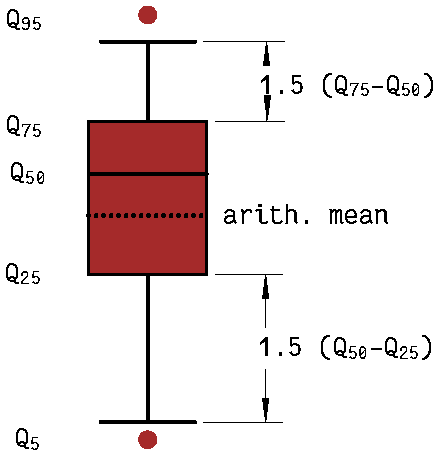
\includegraphics[width=0.25\textwidth]{Graphics/Box-and-Wisker} The quartiles are used also to create \textbf{box-and-whisker plots}, where the box encompasses the interquartile range and the whiskers have the length of \(1.5 (Q_{50}-Q_{25} \) and \(1.5 (Q_{75}-Q_{50}) \), respectively. Data outside the whisker range are considered outliers. They can be placed individually, or the \skalar{Q_5} and \skalar{Q_{95}}-points are marked instead. Marking the arithmetic mean by a dotted line is optional, but gives a good idea about the skew of the data. This plot is very good for comparing data vectors obtained under different experimental conditions for position and spread.

The coefficient of quartile deviation \( \frac{Q3-Q1}{Q3+Q1} \) is another measure of dispersione.

\begin{lstlisting}
  FUNCTION StandardErrorOfMedian(Data: VectorTyp): float;

  VAR
    i, j, n: WORD;

  BEGIN
    n := VectorLength(Data);
    IF (n = 0)
      THEN
        BEGIN
          CH := WriteErrorMessage('Weighted low median from vector of length 0');
          DeskriptError := TRUE;
          EXIT;
        END;
    i := Round(n / 2 - Sqrt(3 * n) / 2);
    j := Round(n / 2 + Sqrt(3 * n) / 2);
    Result := (GetVectorElement(Data, j) - GetVectorElement(Data, i)) / 3.4641;
  END;
\end{lstlisting}

The \acf{MAD} \parencite{Rou-93} is the median of \( |\AbsVec{x}_i - \breve{\AbsVec{x}}| \), a robust measure of dispersion with a breakdown point of \SI{50}{\%} of the data. It is thus more useful than the interquartile distance. To make the \acs{MAD} consistent with other measures of dispersion, it needs to be multiplied by a scaling parameter, to make it consistent with the standard deviation \skalar{\sigma}, this parameter is \( \frac{1}{\sqrt{2}} \mathrm{qnorm}\left(\frac{5}{8}\right) = \num{1.4826} \). To detect outliers in the data vector, one can flag those \( \AbsVec{x}_i \), whose \( \frac{|\AbsVec{x}_i - \breve{\AbsVec{x}}|}{\mathrm{MAD}(\AbsVec{x})} \) exceeds a cutoff, for example \num{2.5} or \num{3.0}. However, this assumes a distribution symmetrical around the median.

\begin{lstlisting}[caption=median absolute deviation from median (MAD)]
  FUNCTION MAD(Data: VectorTyp): double;

  CONST
    Scale = 1.4826; //   1 / (Sqrt(2) * qnorm(5/8))

  VAR
    m, Sum, cn: float;
    n, i: WORD;
    Dev: VectorTyp;

  BEGIN
    n := VectorLength(Data);
    IF (n = 0)
      THEN
        BEGIN
          CH := WriteErrorMessage('MAD from vector of length 0');
          DeskriptError := TRUE;
          EXIT;
        END;
    m := Median(Data);
    CreateVector(Dev, n, 0.0);
    FOR i := 1 TO n DO
      SetVectorElement(Dev, i, Abs(GetVectorElement(Data, i) - m));
    CASE n OF
      2: cn := 1.196;
      3: cn := 1.495;
      4: cn := 1.363;
      5: cn := 1.206;
      6: cn := 1.200;
      7: cn := 1.140;
      8: cn := 1.129;
      9: cn := 1.107
      ELSE
        cn := n / (n - 0.8);
    END; { case }
    MAD := cn * Scale * Median(Dev);
    DestroyVector(Dev);
  END;
\end{lstlisting}

To calculate \acs{MAD} as parameter of dispersion, one first has to calculate \skalar{\breve{\AbsVec{x}}} as parameter of position.

Dispersion parameters corresponding to the \Name{Hodges-Lehmann}-estimator of location are \skalar{S_n} and \skalar{Q_n} \parencite{Rou-93}:
\begin{eqnarray}
  S_n &=& c_n \times 1.1926 \times \mathrm{lomed}_{i = 1\ldots n}\left(\mathrm{himed}_{j \neq i} |\AbsVec{x}_i - \AbsVec{x}_j|\right)\\
  Q_n &=& c_n \times 2.2219 \times [|\AbsVec{x}_i - \AbsVec{x}_j|, i < j]_{(k)}
\end{eqnarray}
The constant factor is for consistency at normal distribution, \skalar{c_n} is a finite sample correction factor. For a maximal breakdown point, \( k = \binom{n}{s}/4 \). For both \skalar{S_n} and \skalar{Q_n}, the breakdown point is \( (n\ \mathrm{div}\ 2)\ \mathrm{div}\ n \), the best possible value \parencite{Cro-92}. \Name{Gauss}ian asymptotic efficiency is \SI{58}{\%} for \skalar{S_n}, and even \SI{82}{\%} for \skalar{Q_n}. If we divide \skalar{Q_n} by \( \sqrt{n} \), we get a robust standard error.

\begin{lstlisting}[caption= naive Sn and Qn: \textbf{O}($n^2$)]
  FUNCTION NaiveSn(VAR Data: VectorTyp): float;

  VAR
    i, j, n: WORD;
    a1, a2: VectorTyp;
    xi, cn: float;

  BEGIN
    n := VectorLength(Data);
    IF (n = 0)
      THEN
        BEGIN
          CH := WriteErrorMessage('Sn from vector of length 0');
          DeskriptError := TRUE;
          EXIT;
        END;
    CreateVector(a1, n, 0.0);
    CreateVector(a2, n, 0.0);
    FOR i := 1 TO n DO
      BEGIN
        xi := GetVectorElement(Data, i);
        FOR j := 1 TO n DO
          SetVectorElement(a1, j, Abs(xi - GetVectorElement(Data, j)));
        ShellSort(a1);
        SetVectorElement(a2, i, GetVectorElement(a1, Succ(n DIV 2))); // high median
      END;
    DestroyVector(a1);
    ShellSort(a2);
    CASE n OF
      2: cn := 0.743;
      3: cn := 1.851;
      4: cn := 0.954;
      5: cn := 1.351;
      6: cn := 0.993;
      7: cn := 1.198;
      8: cn := 1.005;
      9: cn := 1.131
      ELSE IF Odd(n)
             THEN cn := n / (n - 0.9)
             ELSE cn := 1;
    END; { case }
    Result := cn * 1.1926 * GetVectorElement(a2, Succ(n) DIV 2);  // LOW median
  END;



  FUNCTION NaiveQn(VAR Data: VectorTyp): float;

  VAR
    i, j, n, k: WORD;
    a1: VectorTyp;
    xi, dn: float;

  BEGIN
    n := VectorLength(Data);
    IF (n = 0)
      THEN
        BEGIN
          CH := WriteErrorMessage('Qn from vector of length 0');
          DeskriptError := TRUE;
          EXIT;
        END;
    CreateVector(a1, (n - 1) * n DIV 2, 0.0);
    k := 0;
    FOR i := 1 TO n DO
      BEGIN
        xi := GetVectorElement(Data, i);
        FOR j := Succ(i) TO n DO
          BEGIN
            INC(k);
            SetVectorElement(a1, k, Abs(xi - GetVectorElement(Data, j)));
          END;
      END;
    ShellSort(a1);
    CASE n OF   // finite sample correction factor
      2: dn := 0.399;
      3: dn := 0.994;
      4: dn := 0.512;
      5: dn := 0.844;
      6: dn := 0.611;
      7: dn := 0.857;
      8: dn := 0.669;
      9: dn := 0.872;
      ELSE
        IF Odd(n)    // n >= 10
          THEN dn := n / (n + 1.4)
          ELSE dn := n / (n + 3.8);
    END; { case }
    xi := GetVectorElement(a1, Round(BinomialCoef(n, 2)) DIV 4);
    Result := dn * 2.2219 * xi;
    DestroyVector(a1);
  END;
\end{lstlisting}

These algorithms are \textbf{O}(\skalar{n^2}), and the naive Qn implementation is limited to \skalar{n} = 141 by available memory. However, they can be made \textbf{O}(\skalar{n} log(\skalar{n})) with \textbf{O}(\skalar{n}) storage space requirement \parencite{Cro-92}.

\begin{lstlisting}[caption= final Sn: \textbf{O}($n \log(n)$)]
  FUNCTION Sn(VAR Data: VectorTyp): float;

  VAR
    n, i, j, l, nA, nB, rightA, rightB, leftA, leftB, tryA, tryB, diff,
    Amin, Amax, even, half: WORD;
    cn, medA, medB: float;
    a2: VectorTyp;

  BEGIN
    n := VectorLength(Data);
    IF (n = 0)
      THEN
        BEGIN
          CH := WriteErrorMessage('Sn from vector of length 0');
          DeskriptError := TRUE;
          EXIT;
        END;
    ShellSort(Data);
    CreateVector(a2, n, 0.0);
    SetVectorElement(a2, 1, GetVectorElement(Data, Succ(n DIV 2)) -
      GetVectorElement(Data, 1));
    FOR i := 2 TO (Succ(n) DIV 2) DO // a2(i) = lomed_{j<>i} | xi - xj |, i = 2...Succ(n)/2
      BEGIN
        nA := Pred(i);
        nB := n - i;
        diff := nB - nA;
        leftA := 1;
        leftB := 1;
        rightA := nB;
        rightB := nB;
        Amin := Succ(diff DIV 2);
        Amax := diff DIV 2 + nA;
        WHILE (leftA < rightA) DO
          BEGIN
            l := Succ(rightA - leftA);
            even := 1 - (l MOD 2);
            half := Pred(l) DIV 2;
            tryA := leftA + half;
            tryB := leftB + half;
            IF (tryA < Amin)
              THEN
                BEGIN
                  rightB := tryB;
                  leftA := tryA + even;
                END
              ELSE IF (tryA > Amax)
                     THEN
                       BEGIN
                         rightA := tryA;
                         leftB := tryB + even;
                       END
                     ELSE
                       BEGIN
                         medA := GetVectorElement(Data, i) - GetVectorElement(Data, (i - tryA + Amin - 1));
                         medB := GetVectorElement(Data, tryB + i) - GetVectorElement(Data, i);
                         IF (medA >= medB)
                           THEN
                             BEGIN
                               rightA := tryA;
                               leftB := tryB + even;
                             END
                           ELSE
                             BEGIN
                               rightB := tryB;
                               leftA := tryA + even;
                             END;
                       END;
          END; { while }
        IF (leftA > Amax)
          THEN
            SetVectorElement(a2, i, GetVectorElement(Data, leftB + i) -
                             GetVectorElement(Data, i))
          ELSE
            BEGIN
              medA := GetVectorElement(Data, i) - GetVectorElement(Data,
                Pred(i - leftA + Amin));
              medB := GetVectorElement(Data, leftB + i) - GetVectorElement(Data, i);
              SetVectorElement(a2, i, min(medA, medB));
            END;
      END; { for }
    FOR i := Succ(Succ(n) DIV 2) TO Pred(n) DO    // same, but i = Succ(Succ(n)/2) ... n-1
      BEGIN
        nA := n - i;
        nB := Pred(i);
        diff := nB - nA;
        leftA := 1;
        leftB := 1;
        rightA := nB;
        rightB := nB;
        Amin := Succ(diff DIV 2);
        Amax := diff DIV 2 + nA;
        WHILE (leftA < rightA) DO
          BEGIN
            l := Succ(rightA - leftA);
            even := 1 - (l MOD 2);  // 0 OR 1
            half := Pred(l) DIV 2;
            tryA := leftA + half;
            tryB := leftB + half;
            IF (tryA < Amin)
              THEN
                BEGIN
                  rightB := tryB;
                  leftA := tryA + even;
                END
              ELSE IF (tryA > Amax)
                     THEN
                       BEGIN
                         rightA := tryA;
                         leftB := tryB + even;
                       END
                     ELSE
                       BEGIN
                         medA := GetVectorElement(Data, Succ(i + tryA - Amin)) -
                                 GetVectorElement(Data, i);
                         medB := GetVectorElement(Data, i) -
                                 GetVectorElement(Data, i - tryB);
                        IF (medA >= medB)
                          THEN
                            BEGIN
                              rightA := tryA;
                              leftB := tryB + even;
                            END
                          ELSE
                            BEGIN
                              rightB := tryB;
                              leftA := tryA + even;
                            END;
                      END;
          END; { while }
        IF (leftA > Amax)
          THEN
            SetVectorElement(a2, i, GetVectorElement(Data, i) -
                             GetVectorElement(Data, i - leftB))
          ELSE
            BEGIN
              medA := GetVectorElement(Data, Succ(i + leftA - Amin)) -
                      GetVectorElement(Data, i);
              medB := GetVectorElement(Data, i) - GetVectorElement(Data, i - leftB);
              SetVectorElement(a2, i, min(medA, medB));
            END;
      END; { for }
    SetVectorElement(a2, n, GetVectorElement(Data, n) -
      GetVectorElement(Data, Succ(n) DIV 2));
    CASE n OF           // finite sample correction factor
      2: cn := 0.743;
      3: cn := 1.851;
      4: cn := 0.954;
      5: cn := 1.351;
      6: cn := 0.993;
      7: cn := 1.198;
      8: cn := 1.005;
      9: cn := 1.131
      ELSE
        IF Odd(n)
          THEN cn := n / (n - 0.9)
          ELSE cn := 1;
    END; { case }
    ShellSort(a2);
    Result := cn * 1.1926 * GetVectorElement(a2, Succ(n) DIV 2);
    DestroyVector(a2);
  END; { Sn }
\end{lstlisting}

\begin{lstlisting}[caption=Qn: doesn't give same result as naive Qn]
  FUNCTION Qn(VAR Data: VectorTyp): float;

  TYPE
    IntVec = ARRAY [1..MaxVector] OF WORD;

  VAR
    work, weight: VectorTyp;
    Left, Right, Q, P: IntVec;
    n, h, i, j, jj, k, knew, kcand, jhelp, nL, nR, sumQ, sumP: WORD;
    found: BOOLEAN;
    trial, dn: float;

    FUNCTION WeightedHiMedian(SortedData, weight: VectorTyp): float;

    VAR
      acand, iwcand: VectorTyp;
      wrest, wleft, wmid, wright, i, n, nn: WORD;
      wtotal: float;

    BEGIN
      n := VectorLength(SortedData);
      nn := n;
      wtotal := 0;
      CreateVector(acand, n, 0.0);
      CreateVector(iwcand, n, 0.0);
      FOR i := 1 TO nn DO
        wtotal := wtotal + GetVectorElement(weight, i);
      wrest := 0;
      WHILE TRUE DO    // infinite LOOP EXIT'ed when result known
        BEGIN
          Trial := GetVectorElement(SortedData, succ(nn div 2));
          wleft := 0;
          wmid := 0;
          wright := 0;
          FOR i := 1 TO nn DO
            IF (GetVectorElement(SortedData, i) < trial)
              THEN wleft := wleft + trunc(GetVectorElement(weight, i))
              ELSE IF (GetVectorElement(SortedData, i) > trial)
                     THEN wright := wright + trunc(GetVectorElement(weight, i))
                     ELSE wmid := wmid + trunc(GetVectorElement(weight, i));
          IF ((2 * wrest + 2 * wleft) > wtotal)
            THEN
              BEGIN
                kcand := 0;
                FOR i := 1 TO nn DO
                  IF (GetVectorElement(SortedData, i) < trial)
                    THEN
                      BEGIN
                        Inc(kcand);
                        SetVectorElement(acand, kcand, GetVectorElement(SortedData, i));
                        SetVectorElement(iwcand, kcand, GetVectorElement(weight, i));
                      END;
                nn := kcand;
              END
            ELSE
              BEGIN
                IF ((2 * wrest + 2 * wleft + 2 * wmid) > wtotal)  // Endpunkt wird nicht erreicht
                  THEN
                    BEGIN
                      WeightedHiMedian := trial;
                      exit;
                    END
                  ELSE
                    BEGIN
                      kcand := 0;
                      FOR i := 1 TO nn DO
                        IF (GetVectorElement(SortedData, i) > trial)
                          THEN
                            BEGIN
                              Inc(kcand);
                              SetVectorElement(acand, kcand,
                                GetVectorElement(SortedData, i));
                              SetVectorElement(iwcand, kcand,
                                GetVectorElement(weight, i));
                            END;
                      nn := kcand;
                      wrest := wrest + wleft + wmid;
                    END; { else }
              END; { else }
          FOR i := 1 TO nn DO
            BEGIN
              SetVectorElement(SortedData, i, GetVectorElement(acand, i));
              SetVectorElement(weight, i, GetVectorElement(iwcand, i));
            END;
        END; { while }
      DestroyVector(acand);
      DestroyVector(iwcand);
    END;  { WeightedHiMedian }

  BEGIN
    n := VectorLength(Data);
    IF (n = 0)
      THEN
        BEGIN
          ch := WriteErrorMessage('Qn from vector OF Length 0');
          DeskriptError := TRUE;
          EXIT;
        END;
    h := succ(n div 2);
    k := h * pred(h) div 2;
    ShellSort(Data);
    CreateVector(work, n, 0.0);
    CreateVector(weight, n, 0.0);
    FOR i := 1 TO n DO
      BEGIN
        left[i] := n - i + 2;
        right[i] := n;
      END;
    jhelp := n * succ(n) div 2;
    knew := k + jhelp;
    nL := jhelp;
    nR := sqr(n);
    found := False;
    WHILE ((nR - nL > n) and (not found)) DO
      BEGIN
        j := 1;
        FOR i := 2 TO n DO
          IF (left[i] <= right[i])
            THEN
              BEGIN
                SetVectorElement(weight, j, succ(right[i] - left[i]));
                jhelp := left[i] + trunc(GetVectorElement(weight, j)) div 2;
                SetVectorElement(work, j, GetVectorElement(Data, i) -
                  GetVectorElement(Data, succ(n) - jhelp));
                Inc(j);
              END;
        trial := WeightedHiMedian(work, weight);
        j := 0;
        FOR i := n DOWNTO 1 DO
          BEGIN
            WHILE ((j < n) AND (GetVectorElement(Data, i) - GetVectorElement(Data, n - j)
                 < trial)) DO
              Inc(j);
            P[i] := j;
          END;
        j := succ(n);
        FOR i := 1 TO n DO
          BEGIN
            WHILE (GetVectorElement(Data, i) - GetVectorElement(Data, n - j + 2) > trial) DO
              Dec(j);
            Q[i] := j;
          End;
        sumP := 0;
        sumQ := 0;
        FOR i := 1 TO n DO
          BEGIN
            sumP := sumP + P[i];
            sumQ := sumQ + pred(Q[i]);
          END;
        IF (knew <= sumP)     // problem about here
          THEN
            BEGIN
              FOR i := 1 TO n DO
                right[i] := P[i];
              nR := sumP;
            END
          ELSE IF (knew > sumQ)
                 THEN
                   BEGIN
                     FOR i := 1 TO n DO
                       left[i] := Q[i];
                     nL := sumQ;
                   END
                 ELSE
                   BEGIN
                     Qn := trial;
                     found := True;
                   END;
      END; { WHILE }
    IF NOT (found)
      THEN
        BEGIN
          j := 1;
          FOR i := 2 TO n DO
            IF (left[i] <= right[i])
              THEN
                FOR jj := left[i] TO right[i] DO
                  BEGIN
                    SetVectorElement(work, j, GetVectorElement(Data, i) -
                      GetVectorElement(Data, succ(n - jj)));
                    Inc(j);  // !!!! grows bejond n !!!!
                  END;
        END;
    CASE n OF   // finite sample correction factor
      2: dn := 0.399;
      3: dn := 0.994;
      4: dn := 0.512;
      5: dn := 0.844;
      6: dn := 0.611;
      7: dn := 0.857;
      8: dn := 0.669;
      9: dn := 0.872;
      ELSE
        IF odd(n)
          THEN dn := n / (n + 1.4)
          ELSE dn := n / (n + 3.8);
    END; { case }
    ShellSort(work);
    Result := dn * 2.2219 * GetVectorElement(work, knew - nL);
    DestroyVector(work);
    DestroyVector(weight);
  END;
\end{lstlisting}

\subsubsection{L-moments}

The non-parametric equivalent of the \Name{Pearson}-moments are the L-moments. For an increasing ordered sample vector the \skalar{r}th L-moment is
\begin{equation}
   \lambda_r = r^{-1} \binom{n}{r}^{-1} \sum_{x_1 < \ldots < x_j < \ldots < x_r}{(-1)^{r-j} \binom{r-1}{j} \AbsVec{x}_j}
\end{equation}
This means that
\begin{eqnarray}
  \ell_1 &=& \binom{n}{1}^{-1} \sum_{i=1}^n{\AbsVec{x}_i}  = n^{-1} \sum_{i=1}^n{\AbsVec{x}_i} \\
  \nonumber
  \ell_2 &=& \frac{1}{2} \binom{n}{2}^{-1} \sum_{i=1}^n{\left[\binom{i-1}{1} - \binom{n-i}{1}\right] \AbsVec{x}_{(i)}} \\
  \nonumber
         &=& \frac{1}{(n-1) n} \sum_{i=1}^n{(2i - n -1) \AbsVec{x}_{(i)}}\\
  \nonumber
  \ell_3 &=& \frac{1}{3} \binom{n}{3}^{-1} \sum_{i=1}^n{\left[\binom{i-1}{2} - 2 \binom{i-1}{1}\binom{n-i}{1} + \binom{n-i}{2}\right]\AbsVec{x}_{(i)}} \\
  \nonumber
         &=& \frac{2}{n^3 - 3n^2 + 2n} \sum_{i=1}^n{\left[3i^2 - 3in - 3i + \frac{n^2}{2} + \frac{3n}{2} + 1  \right]\AbsVec{x}_{(i)}}\\
  \nonumber
  \ell_4 &=& \frac{1}{4} \binom{n}{4}^{-1} \sum_{i=1}^n{\left[\binom{i-1}{3} - 3 \binom{i-1}{2}\binom{n-i}{1} + 3 \binom{i-1}{1}\binom{n-i}{2} - \binom{n-i}{3}\right]\AbsVec{x}_{(i)}} \\
  \nonumber
         &=& \frac{6}{n^4 - 6n^3 + 11n^2 - 6n} \sum_{i=1}^n{\left[\frac{10 i^3}{3} - 5 i^2 n - 5 i^2 + 2 i n^2 + 5 i n + \frac{11 i}{3} - \frac{n^3}{6} - n^2 - \frac{11 n}{6} - i\right]\AbsVec{x}_{(i)}}
\end{eqnarray}
where \skalar{\AbsVec{x}_{(i)}} is the \skalar{i}th order statistics (\skalar{i}th smallest value) of the data vector. The first two L-moments have conventional names:
\begin{description}
  \item[\(\ell_1\)]{L-mean (identical to arithmetic mean)}
  \item[\(\ell_2\)]{L-dispersion (half the mean absolute difference)}
\end{description}
L-moments, when standardised, are called
\begin{description}
  \item[\(\tau_2 = \ell_2/\ell_1\)]{coefficient of L-variation (identical to \Name{Gini}-coefficient)}
  \item[\(\tau_3 = \ell_3/\ell_2\)]{L-skewness}
  \item[\(\tau_4 = \ell_4/\ell_2\)]{L-kurtosis}
\end{description}
L-moments are more robust against outliers than conventional moments, and may exist for distributions where conventional moments cannot be defined (they require only a finite mean). For \textbf{Trimmed L-moments}, extreme values are left out during calculation for additional robustness.



\begin{lstlisting}[caption=L-moments]
  FUNCTION Ell2(CONST SortedData: VectorTyp): float;

  VAR
    sum, factor: float;
    i, n: WORD;

  BEGIN
    n := VectorLength(SortedData);
    IF (n = 0)
      THEN
        BEGIN
          CH := WriteErrorMessage('Ell2 from vector OF Length 0');
          DeskriptError := TRUE;
          EXIT;
        END;
    sum := 0;
    FOR i := 1 TO n DO
      BEGIN
        factor := Pred(2 * i - n);
        sum := sum + factor * GetVectorElement(SortedData, i);
      END;
    Factor := 1 / (n * n - n);
    Result := Factor * Sum;
  END;

  FUNCTION Ell3(CONST SortedData: VectorTyp): float;

  VAR
    sum, factor: float;
    i, n: WORD;

  BEGIN
    n := VectorLength(SortedData);
    IF (n = 0)
      THEN
        BEGIN
          CH := WriteErrorMessage('Ell3 from vector OF Length 0');
          DeskriptError := TRUE;
          EXIT;
        END;
    sum := 0;
    FOR i := 1 TO n DO
      BEGIN
        factor := 3 * i * i - 3 * i * n - 3 * i + n * n / 2 + 3 * n / 2 + 1;
        sum := sum + factor * GetVectorElement(SortedData, i);
      END;
    Factor := 2 / (n * n * n - 3 * n * n + 2 * n);
    Result := Factor * Sum;
  END;


  FUNCTION Ell4(CONST SortedData: VectorTyp): float;

  VAR
    sum, factor: float;
    i, n: WORD;

  BEGIN
    n := VectorLength(SortedData);
    IF (n = 0)
      THEN
        BEGIN
          CH := WriteErrorMessage('Ell4 from vector OF Length 0');
          DeskriptError := TRUE;
          EXIT;
        END;
    sum := 0;
    FOR i := 1 TO n DO
      BEGIN
        factor := 10 * i * i * i / 3 - 5 * i * i * n - 5 * i * i + 2 * i * n * n + 5 * i * n +
          11 * i / 3 - n * n * n / 6 - n * n - 11 * n / 6 - i;
        sum := sum + factor * GetVectorElement(SortedData, i);
      END;
    Factor := 6 / (n * n * n * n - 6 * n * n * n + 11 * n * n - 6 * n);
    Result := Factor * Sum;
  END;
\end{lstlisting}

\paragraph{Other moments}

\Name{Bowley}'s measure of skewness \parencite{Bow-01} is \( Q1 - 2 Q2 + Q3 \), in effect the difference between the upper and lower part of the box in a box-and-whisker plot. It is an absolute measure of skewness in the units of the data. It can therefore not be used to compare the skewness of two vectors that, say, measured weight and height of individuals. For that purpose, the dimensionless relative skewness is used \( \gamma_B = \frac{Q1 - 2Q2 + Q3}{(Q3 - Q1)} \), which is bounded between [-1\ldots 1]. \Name{Kelly}'s definition uses the \num{10} and \SI{90}{\%} quantiles rather than Q2 and Q3 as limits, thereby using more of the data. Fundamentally, of course, one can set the limits quite arbitrarily \parencite{Yul-29}.

\begin{lstlisting}
FUNCTION QuartileCoefficientOfSkewness(Q1, Q2, Q3: float): float;

BEGIN
  Result := (Q1 - 2 * Q2 + Q3) / (Q3 - Q1);
END;
\end{lstlisting}

The percentile coefficient of kurtosis compares the width of the curves for the central \SI{50}{\%} of the data with the width of the middle \SI{80}{\%}. Again, it is possible to use even wider ranges, but then the result should be scaled so that the kurtosis of the normal distribution is unity (\num{1}-\SI{99}{\%} s = 1/3.49).

\begin{lstlisting}
  FUNCTION CentilCoeffKurtosis(Data: VectorTyp): float;

  VAR
    Q1, Q3, Q10, Q90: float;
    n: WORD;

  BEGIN
    n := VectorLength(Data);
    IF (n = 0)
      THEN
        BEGIN
          CH := WriteErrorMessage('Centile coefficient OF kurtosis from vector OF Length 0');
          DeskriptError := TRUE;
          EXIT;
        END;
    Q1 := Quantile(Data, 0.25);
    Q3 := Quantile(Data, 0.75);
    Q10 := Quantile(Data, 0.10);
    Q90 := Quantile(Data, 0.90);
    Result := 0.5 * (Q3 - Q1) / (Q90 - Q10);
  END;
\end{lstlisting}

\section{Normalisation and standardisation of vectors}

The following routine centers a vector to mean zero by subtracting from each element the average:
\begin{equation}
  \AbsVec{c}_{i} = \AbsVec{x}_{i} - \bar{\AbsVec{x}}
\end{equation}

\begin{lstlisting}
  PROCEDURE MeanNormalise(VAR Data: VectorTyp);

  VAR
    Mean: double;
    i, n: WORD;

  BEGIN
    n := VectorLength(Data);
    IF (n = 0)
      THEN
        BEGIN
          CH := WriteErrorMessage('Normalisation OF vector OF Length 0');
          DeskriptError := TRUE;
          EXIT;
        END;
    Mean := ArithmeticMean(Data);
    FOR i := 1 TO VectorLength(Data) DO
      SetVectorElement(Data, i, (GetVectorElement(Data, i) - Mean));
  END;
\end{lstlisting}

\skalar{z}-standardising data works like centring, except that the data are also normalised to a standard deviation of \num{1.0}:
\begin{equation}
  \AbsVec{z}_{i} = \frac{\AbsVec{x}_{i} - \bar{\AbsVec{x}}}{s(\AbsVec{a})}
\end{equation}

\begin{lstlisting}
  PROCEDURE Z_Standardise(VAR Data: VectorTyp);

  VAR
    Mean, s: double;
    i, n: WORD;

  BEGIN
    n := VectorLength(Data);
    IF (n = 0)
      THEN
        BEGIN
          CH := WriteErrorMessage('Standardisation OF vector OF Length 0');
          DeskriptError := TRUE;
          EXIT;
        END;
    Mean := ArithmeticMean(Data);
    s := StandardDeviation(Data);
    FOR i := 1 TO n DO
      SetVectorElement(Data, i, (GetVectorElement(Data, i) - Mean) / s);
  END;
\end{lstlisting}

Robust standardisation is performed essentially as \skalar{z}-standardisation, however, instead of the mean the median is subtracted from the data, and the data are divided by \skalar{Q_n} rather than the standard deviation. Note that the routine for calculating the median sorts the data, which would be a problem if used on the columns of a matrix. Therefore, the calculation of median and \skalar{Q_n} are performed on a copy of the data vector.

\begin{lstlisting}
  PROCEDURE RobustStandardise(VAR Data: VectorTyp);

  VAR
    Mean, s: double;
    i, n: WORD;
    Sorted: VectorTyp;

  BEGIN
    n := VectorLength(Data);
    IF (n = 0)
      THEN
        BEGIN
          CH := WriteErrorMessage('Standardisation OF a vector OF Length 0');
          DeskriptError := TRUE;
          EXIT;
        END;
    CopyVector(Data, Sorted);
    Mean := Median(Sorted);  // so that order OF elements IS NOT changed
    s := NaiveQn(Sorted);
    FOR i := 1 TO n DO
      SetVectorElement(Data, i, (GetVectorElement(Data, i) - Mean) / s);
    DestroyVector(Sorted);
  END;
\end{lstlisting}


\section{Grouped data}

\begin{lstlisting}
  FUNCTION WeightedMean(Means, Vars, Lengths: VectorTyp): float;

  VAR
    Sum1, Sum2: float;
    i, n: WORD;

  BEGIN
    Sum1 := 0;
    Sum2 := 0;
    n := VectorLength(Means);
    IF (n = 0)
      THEN
        BEGIN
          CH := WriteErrorMessage('Weighted mean from vector of length 0');
          DeskriptError := TRUE;
          EXIT;
        END;
    FOR i := 1 TO n DO
      BEGIN
        Sum1 := Sum1 + (GetVectorElement(Lengths, i) * GetVectorElement(Means, i) /
                        GetVectorElement(Vars, i));
        Sum2 := Sum2 + (GetVectorElement(Lengths, i) / GetVectorElement(Vars, i));
      END;
    Result := Sum1 / Sum2;
  END;
\end{lstlisting}


\begin{lstlisting}
  FUNCTION WeightedStandardDeviation(Means, Vars, Lengths: VectorTyp): float;

  VAR
    Sum1, Sum2: float;
    i, n: WORD;

  BEGIN
    Sum1 := 0;
    Sum2 := 0;
    n := VectorLength(Means);
    IF (n = 0)
      THEN
        BEGIN
          CH := WriteErrorMessage('Weighted standard deviation from vector of length 0');
          DeskriptError := TRUE;
          EXIT;
        END;
    FOR i := 1 TO n DO
      BEGIN
        Sum1 := Sum1 + (GetVectorElement(Lengths, i) - 1) * GetVectorElement(Vars, i);
        Sum2 := Sum2 + GetVectorElement(Lengths, i);
      END;
    Result := Sum1 / (Sum2 - n);
  END;
\end{lstlisting}

\section{Descriptive statistics of matrices}

\subsubsection{Variance-covariance matrix}

The following routine to calculate the variance-covariance matrix \arr{S} is robust against missing data, but does not guarantee a positive-definite result. It calculates the matrix by calculating the covariance of all pairs of data vectors:

\begin{lstlisting}[caption=Variance-covariance matrix]
  PROCEDURE VarCovarMatrix(CONST Data: MatrixTyp; VAR VarCovar: MatrixTyp);

  VAR
    Rows, Columns, i, j: WORD;
    x, y: VectorTyp;

  BEGIN
    Rows := MatrixRows(Data);
    Columns := MatrixColumns(Data);
    CreateMatrix(VarCovar, Columns, Columns, 0.0);
    FOR i := 1 TO Columns DO
      BEGIN
        GetColumn(Data, i, x);
        SetMatrixElement(VarCovar, i, i, Covariance(x, x));
        FOR j := Succ(i) TO Columns DO
          BEGIN
            GetColumn(Data, j, y);
            SetMatrixElement(VarCovar, i, j, Covariance(x, y));
            SetMatrixElement(VarCovar, j, i, GetMatrixElement(VarCovar, i, j));
            DestroyVector(y);
          END;
        DestroyVector(x);
      END;
  END;
\end{lstlisting}

The following routine also calculates \arr{S}, but uses a matrix approach. This ensures a positive definite result, but cannot handle missing data.

\begin{lstlisting}[caption=Variance-covariance matrix]
  PROCEDURE VarCov(CONST Data: MatrixTyp; VAR VarCovar: MatrixTyp);

  VAR
    Columns, Rows: WORD;
    Ones, I1, Dev, DevT: MatrixTyp;

  BEGIN
    Rows := MatrixRows(Data);
    Columns := MatrixColumns(Data);
    CreateMatrix(Ones, Rows, Rows, 1.0);
    MatrixInnerProduct(Ones, Data, I1);
    SkalarMultiplikation(I1, 1 / Rows);
    NegativeMatrix(I1);
    MatrixAdd(Data, I1, Dev);          // deviation scores
    DestroyMatrix(I1);
    DestroyMatrix(Ones);
    MatrixTranspose(Dev, DevT);
    MatrixInnerProduct(DevT, Dev, VarCovar); // deviation score sum OF squares
    SkalarMultiplikation(VarCovar, 1 / Pred(Rows));
    DestroyMatrix(Dev);
    DestroyMatrix(DevT);
  END;
\end{lstlisting}

\subsubsection{Mean and standard deviation of columns}

\begin{lstlisting}[caption=Column means of a matrix]
  PROCEDURE MeanVector(CONST Data: MatrixTyp; VAR Mean: VectorTyp);

  VAR
    Columns, i, j: WORD;
    x: VectorTyp;

  BEGIN
    Columns := MatrixColumns(Data);
    CreateVector(Mean, Columns, 0.0);
    FOR j := 1 TO Columns DO
      BEGIN
        GetColumn(Data, j, x);
        SetVectorElement(Mean, j, NeumaierSum(x) / ActualElements(x)); // arithmetic mean
        DestroyVector(x);
      END;
  END;
\end{lstlisting}


\begin{lstlisting}[caption=Column standard deviation of a matrix]
  PROCEDURE StaVector(CONST Data: MatrixTyp; VAR Sta: VectorTyp);

  VAR
    Columns, Rows, i, j: WORD;
    x: VectorTyp;

  BEGIN
    Rows := MatrixRows(Data);
    Columns := MatrixColumns(Data);
    CreateVector(Sta, Columns, 0.0);
    FOR j := 1 TO Columns DO
      BEGIN
        GetColumn(Data, j, x);
        SetVectorElement(Sta, j, StandardDeviation(x));
        DestroyVector(x);
      END;
  END;
\end{lstlisting}

\subsubsection{Matrix standardisation and normalisation}


\begin{lstlisting}[caption=]
  PROCEDURE CentreMatrix(VAR A: MatrixTyp);

  VAR
    Data: VectorTyp;
    j, Columns: WORD;

  BEGIN
    Columns := MatrixColumns(A);
    FOR j := 1 TO Columns DO
      BEGIN
        GetColumn(A, j, Data);
        Centre(Data);
        SetColumn(A, Data, j);
        DestroyVector(Data);
      END;
  END;

  PROCEDURE StandardiseMatrix(VAR A: MatrixTyp);

  VAR
    Data: VectorTyp;
    j, Columns: WORD;

  BEGIN
    Columns := MatrixColumns(A);
    FOR j := 1 TO Columns DO
      BEGIN
        GetColumn(A, j, Data);
        Z_Standardise(Data);
        SetColumn(A, Data, j);
        DestroyVector(Data);
      END;
  END;

  PROCEDURE RobustStandardiseMatrix(VAR A: MatrixTyp);

  VAR
    Data: VectorTyp;
    j, Columns: WORD;

  BEGIN
    Columns := MatrixColumns(A);
    FOR j := 1 TO Columns DO
      BEGIN
        GetColumn(A, j, Data);
        RobustStandardise(Data);
        SetColumn(A, Data, j);
        DestroyVector(Data);
      END;
  END;
\end{lstlisting}

\subsubsection{The \Name{Mahalanobis}-distance \skalar{D_m}}

In multi-dimensional (uncorrelated) data, the distance of a point from the centre of the data cloud could be calculated as \Name{Euklid}ian distance. However, there are several problems:
\begin{itemize}
  \item{If the vectors have different units, what would be the unit of the distance? We would be comparing apples and oranges.}
  \item{If the variables have different scales, the larger variables would influence the result more than the smaller.}
  \item{If the variables have different standard deviations, the less reliable ones should receive smaller weight.}
\end{itemize}
If instead of the variables themself we used their \skalar{z}-scores for distance calculation, these objections would vanish, they are dimensionless, scaled in standard deviations, and more variable factors are given less weight \parencite{War-11}:
\begin{equation}\label{eqn:Maha}
  d_w = \sqrt{z_1^2 + z_2^2 + \ldots z_p^2} = \sqrt{\left(\frac{x_1 - \mu_1}{\sigma_1}\right)^2 + \left(\frac{x_2 - \mu_2}{\sigma_2}\right)^2 + \ldots + \left(\frac{x_p - \mu_p}{\sigma_p}\right)^2}
\end{equation}
If we use the identity matrix instead of the variance-covariance matrix, we get the \Name{Euklid}ian distance.

Squaring both sides and then dividing by \skalar{d_w^2} gives the equation of an ellipsoid around \(\mu \), the vector of their column means:
\begin{equation}
  1 = \frac{(x_1 - \mu_1)^2}{\sigma_1^2 d_w^2} + \frac{(x_2 - \mu_2)^2}{\sigma_2^2 d_w^2} + \ldots + \frac{(x_p - \mu_p)^2}{\sigma_p^2 d_w^2}
\end{equation}
All points on such an \textbf{probability density contour} are equally ``close'' to \(\mu \). Vectorisation and allowing the variables to be correlated gives the \Name{Mahalanobis}-distance \skalar{D_m} \parencite{Mah-36}:
\begin{equation}
  D_m(\AbsVec{x}) = \sqrt{(\AbsVec{x} - \mu) \arr{S}^{-1} (\AbsVec{x} - \mu)^T}
\end{equation}
Note that in some textbooks \AbsVec{x} is defined as column vector, then the transposition needs to be done with the first rather than the third term.

The probability for a \skalar{D_m^2} follows the \(\chi^2 \)-distribution with \skalar{p} degrees of freedom: All points satisfying \(D_m^2 \leq \chi^2(\alpha) \) have a probability \(1 - \alpha \).

The problem with the \Name{Mahalanobis}-distance for identification of outliers is that both the mean vector \(\mu \) and the variance-covariance matrix \arr{S} are influenced by outliers. Instead of the vector of arithmetic means one may use the vector of medians to define a more robust centroid. Another method is to calculate the \Name{Mahalanobis}-distance of each point from the centroid by using \(\mu \) and \arr{S} calculated from the other \(n-1 \) cases. Thus, if the datum under test were an outlier, it would not influence their calculation. However, for very large numbers of cases, the calculation of \skalar{n} inverses of \skalar{n} variance-covariance matrices may be impractical.

The \Name{Mahalanobis}-distance is asymptotically distributed as \(\chi^2_d \). \arr{S} is the sample covariance matrix, in this context also called shape matrix. If \(\beta \) denotes a constant probability level with \(0 \leq \beta \leq 1 \), then the probability of a random variable \(z \sim \chi^2_d \) being greater or equal to \(\chi^2_\beta \) is smaller than
\begin{equation}
   P(z \leq \chi^2_\beta) = 1 - \beta = \alpha
\end{equation}
where \(\alpha \) is called the significance level. Then the cutoff for the \Name{Mahalanobis}-distance becomes \(L_\beta = \sqrt{\chi^2_{d,\beta}} \). Any vector \(\AbsVec{x}_i \) with \(D_i \geq \sqrt{\chi^2_{d;1-\alpha}} \) is a suspected outlier. The \texttt{R}-function \texttt{drawMahal} from the \texttt{chemometrics} package can draw ellipses of constant \skalar{D} into a data set.

\paragraph{Example:}

The data on age, length, weight and lead content of a fish (\Species{Mercurio peces}) population were obtained from \href{https://www.r-bloggers.com/mahalanobis-distance-with-r-exercice/}{https://www.r-bloggers.com/mahalanobis-distance-with-r-exercice/}, accessed 2018-11-19.
\begin{gather} \AbsVec{x} =
  \begin{pmatrix*}[r]
     28 & 31 & 130.0 &  68.12 \\
     24 & 28 & 143.0 & 127.89 \\
     28 & 20 & 136.0 &  89.03 \\
     32 & 34 & 130.5 &  78.28 \\
     22 & 15 & 125.0 & 134.08 \\
     26 & 37 & 147.5 & 135.31 \\
     24 & 19 & 135.0 & 130.48 \\
     28 & 22 & 125.0 &  86.48 \\
     24 & 26 & 127.0 & 129.47 \\
     30 & 21 & 139.0 &  82.43 \\
     22 & 20 & 121.5 & 127.41 \\
     30 & 38 & 150.5 &  71.21 \\
     24 & 17 & 120.0 & 132.06 \\
     26 & 20 & 125.0 &  90.85
  \end{pmatrix*}
\end{gather}
Then
\begin{gather} \mu =
  \begin{pmatrix}
   26.3 & 24.9 & 132.5 & 105.9
  \end{pmatrix}
  \quad \arr{S} =
 \begin{pmatrix*}[r]
    9.76 &  12.81 &  12.08 & -72.15 \\
   12.81 &  56.90 &  49.12 & -70.62 \\
   12.08 &  49.12 &  92.81 & -46.07 \\
  -72.15 & -70.62 & -46.07 & 714.00
 \end{pmatrix*}
 \\ \quad \arr{S}^{-1} =
  \begin{pmatrix*}[r]
    0.5837 & -0.0418 & -0.0275 &  0.0531 \\
   -0.0418 &  0.0390 & -0.0159 & -0.0014 \\
   -0.0275 & -0.0159 &  0.0213 & -0.0030 \\
    0.0531 & -0.0014 & -0.0030 &  0.0064
  \end{pmatrix*}
\end{gather}
Centralisation of the data matrix yields
\begin{gather} (\AbsVec{x} - \mu) =
  \begin{pmatrix*}[r]
     1.71 &  6.14 &  -2.50 & -37.82 \\
    -2.29 &  3.14 &  10.50 &  21.95 \\
     1.71 & -4.86 &   3.50 & -16.91 \\
     5.71 &  9.14 &  -2.00 & -27.66 \\
    -4.29 & -9.86 &  -7.50 &  28.14 \\
    -0.29 & 12.14 &  15.00 &  29.37 \\
    -2.29 & -5.86 &   2.50 &  24.54 \\
     1.71 & -2.86 &  -7.50 & -19.46 \\
    -2.29 &  1.14 &  -5.50 &  23.53 \\
     3.71 & -3.86 &   6.50 & -23.51 \\
    -4.29 & -4.86 & -11.00 &  21.47 \\
     3.71 & 13.14 &  18.00 & -34.73 \\
    -2.29 & -7.86 & -12.50 &  26.12 \\
    -0.29 & -4.86 &  -7.50 & -15.09
  \end{pmatrix*}
\end{gather}
and the product \((\AbsVec{x} - \mu) \arr{S}^{-1} \) becomes
\begin{gather}
  \begin{pmatrix*}[r]
    -1.195 &  0.260 & -0.085 & -0.153 \\
    -0.589 &  0.021 &  0.171 & -0.016 \\
     0.210 & -0.293 &  0.155 & -0.021 \\
     1.541 &  0.188 & -0.263 &  0.119 \\
    -0.390 & -0.125 &  0.031 & -0.010 \\
     0.472 &  0.206 &  0.047 &  0.112 \\
     0.144 & -0.206 &  0.136 &  0.037 \\
     0.294 & -0.037 & -0.103 & -0.008 \\
     0.018 &  0.195 & -0.142 &  0.045 \\
     0.903 & -0.376 &  0.167 &  0.032 \\
    -0.856 &  0.135 & -0.103 & -0.050 \\
    -0.720 &  0.120 &  0.176 & -0.098 \\
     0.724 & -0.049 & -0.156 &  0.095 \\
    -0.558 & -0.037 & -0.030 & -0.083
  \end{pmatrix*}
\end{gather}
Multiplying this result with \((\AbsVec{x} - \mu)^T \) yields

\begin{gather} (\AbsVec{x} - \mu) \arr{S}^{-1} (\AbsVec{x} - \mu)^T = \\
  \begin{pmatrix*}[r]
     5.57 & -0.71  & -1.01 & -0.03 & -1.12 & -2.28 & -2.77 &  0.84 & -0.11 & -2.38 &  1.50 &  2.78 & -2.25 &  2.04 \\
    -0.71 &  2.87  & -0.24 & -3.08 &  0.60 &  2.53 &  1.27 & -2.04 &  0.06 & -0.79 &  0.21 &  1.71 & -1.36 & -0.98 \\
    -1.01 & -0.25  &  2.69 & -1.19 &  0.22 & -1.92 &  1.10 &  0.45 & -2.17 &  3.42 & -1.64 &  0.46 & -0.67 &  0.53 \\
    -0.04 & -3.09  & -1.20 &  7.76 & -3.15 &  1.38 & -2.37 &  1.76 &  0.92 &  0.50 & -2.09 & -0.66 &  1.38 & -1.18 \\
    -1.12 &  0.60  &  0.22 & -3.14 &  2.38 & -1.24 &  1.45 & -0.34 &  0.34 & -0.52 &  1.72 & -2.17 &  1.22 &  0.64 \\
    -2.29 &  2.52  & -1.93 &  1.38 & -1.25 &  6.36 &  0.58 & -2.32 &  1.54 & -1.38 & -1.13 &  1.40 & -0.35 & -3.18 \\
    -2.77 &  1.27  &  1.10 & -2.37 &  1.45 &  0.59 &  2.13 & -0.91 & -0.44 &  1.34 & -0.31 & -1.03 &  0.57 & -0.62 \\
     0.83 & -2.05  &  0.45 &  1.77 & -0.34 & -2.32 & -0.91 &  1.54 & -0.33 &  0.74 & -0.11 & -0.98 &  0.70 &  0.99 \\
    -0.12 &  0.06  & -2.17 &  0.93 &  0.33 &  1.54 & -0.44 & -0.33 &  2.02 & -2.66 &  1.50 & -1.50 &  1.38 & -0.56 \\
    -2.39 & -0.79  &  3.42 &  0.50 & -0.52 & -1.38 &  1.34 &  0.74 & -2.66 &  5.14 & -3.20 &  0.31 & -0.37 & -0.17 \\
     1.50 &  0.21  & -1.64 & -2.08 &  1.72 & -1.13 & -0.31 & -0.11 &  1.51 & -3.20 &  3.08 & -1.53 &  0.89 &  1.12 \\
     2.78 &  1.71  &  0.46 & -0.65 & -2.17 &  1.41 & -1.02 & -0.98 & -1.49 &  0.32 & -1.53 &  5.47 & -4.05 & -0.21 \\
    -2.26 & -1.37  & -0.68 &  1.38 &  1.21 & -0.35 &  0.56 &  0.70 &  1.38 & -0.37 &  0.88 & -4.06 &  3.15 & -0.24 \\
     2.04 & -0.98  &  0.53 & -1.17 &  0.65 & -3.18 & -0.62 &  0.99 & -0.56 & -0.17 &  1.12 & -0.21 & -0.23 &  1.82
  \end{pmatrix*}
\end{gather}

The diagonal elements are \(D_m^2(\AbsVec{x}) \), the square root then is \(D_m(\AbsVec{x}) \):
\begin{gather} D_m^2(\AbsVec{x}) =
  \begin{pmatrix}
     5.57 \\
     2.87 \\
     2.69 \\
     7.76 \\
     2.38 \\
     6.36 \\
     2.13 \\
     1.54 \\
     2.02 \\
     5.14 \\
     3.08 \\
     5.47 \\
     3.15 \\
     1.82
  \end{pmatrix}
  \quad D_m(\AbsVec{x}) =
  \begin{pmatrix}
     2.36 \\
     1.69 \\
     1.64 \\
     2.79 \\
     1.54 \\
     2.52 \\
     1.46 \\
     1.24 \\
     1.42 \\
     2.27 \\
     1.76 \\
     2.34 \\
     1.78 \\
     1.35
  \end{pmatrix}
\end{gather}


\begin{lstlisting}[caption=\Name{Mahalanobis} distance]
  PROCEDURE MahalanobisDistance(CONST Data: MatrixTyp; VAR Dm: VectorTyp);

  VAR
    S, T, C, Inter, Res: MatrixTyp;
    Mean: VectorTyp;
    i, j, Rows, Columns: WORD;
    Sum: float;

  BEGIN
    Rows := MatrixRows(Data);
    Columns := MatrixColumns(Data);
    CreateVector(Dm, Rows, 0.0);
    CreateMatrix(C, Rows, Columns, 0.0);
    MeanVector(Data, Mean);
    VarCovarMatrix(Data, S);
    InverseMatrix(S);
    FOR i := 1 TO Rows DO                  // (x-µ)
      FOR j := 1 TO Columns DO
        SetMatrixElement(C, i, j, GetMatrixElement(Data, i, j) -
          GetVectorElement(Mean, j));
    MatrixTranspose(C, T);                 // (x-µ)^T
    MatrixInnerProduct(C, S, Inter);       // (x-µ) S^-1
    MatrixInnerProduct(Inter, T, Res);     // (x-µ) S^-1 (x-µ)^T
    FOR j := 1 TO Rows DO                  // Sqrt OF diagonal elements
      SetVectorElement(Dm, j, Sqrt(GetMatrixElement(Res, j, j)));
    DestroyMatrix(S);
    DestroyMatrix(T);
    DestroyMatrix(C);
    DestroyMatrix(Inter);
    DestroyMatrix(Res);
    DestroyVector(Mean);
  END;
\end{lstlisting}

\subsubsection{Penalised \Name{Mahalanobis} distance}

Calculating the \Name{Mahalanobis} distance requires the calculation of \(\arr{S}^{-1}(\arr{X}) \).  For a data matrix \(\arr{X}_{n\times p} \) with \(n \geq p \) and rank \(r = \mathrm{rk}(\arr{S}_{p\times p}) < p \) the variance-covariance matrix will not be invertible. This happens if some variables are linear combinations of others, that is, there are actually fewer variables present than \skalar{p}. Then singular value decomposition yields
\begin{eqnarray}
  \arr{S}(\arr{X}) &=& \arr{X}^T\arr{X} \\
  \svd(\arr{X}^T\arr{X})  &=& \arr{V} \Sigma^2 \arr{V}^T = \arr{VDV}^T \quad (\arr{D} = \Sigma^2)
\end{eqnarray}
where \arr{V} and \(\Sigma \) are identical to those of svd(\arr{X}). Thus, in case of a singular variance-covariance matrix \arr{S} the following procedure can be used:
\begin{enumerate}
  \item{center data columns on \(\bar{\AbsVec{x}} \) to calculate the penalised \Name{Mahalanobis} distance. However, it is better to omit this step to calculate the \Name{Euklid}ian distance when data values around 0 contribute least to the classification problem. Then centralising will make nearest-neighbour solutions worse.}
  \item{Calculate the variance-covariance \(\arr{S}(\arr{X}) = \arr{X}^T\arr{X} \).}
  \item{calculate either the svd(\arr{X}) or, if the table is too large, the svd(\arr{S}) (both should be identical).}
  \item{identify the first \skalar{r} significant singular values and calculate \(\AbsVec{d}_i = \sigma_i^2 \)}
  \item{calculate \[\arr{X}_\mathrm{trans} = \arr{V}_{n\times r} \diag{\left(\sqrt{\frac{\AbsVec{d}_i}{\AbsVec{d}_i \sigma}}\right)}\], that is, data weighted by the sqrt-term. }
  \item{Calculate the \Name{Euklid}ian distance of data points in the transformed matrix.}
\end{enumerate}
Alternatively, one could use the \Name{Moore-Penrose} pseudoinverse \(\arr{S}^+ \) to calculate a \Name{Mahalanobis}-like distance (see section \ref{text:pseudoinv} on page \pageref{text:pseudoinv}).

\subsubsection{Robust distance for outlier identification}

\begin{figure}
 \caption{Distance-distance plot. \emph{Top left}: An artificial data set of \num{350} items of two variables with \( \bar{\AbsVec{x}} = \num{110}\pm\num{3}, \bar{\AbsVec{y}} = \num{160}\pm\num{3} \)  (\emph{dark red}) is polluted with \SI{10}{\%} outliers with  \( \bar{\AbsVec{x}} = \num{160}\pm\num{3}, \bar{\AbsVec{y}} = \num{110}\pm\num{3} \) (\emph{green}). Both are clearly separated (\emph{left}). The robust distances calculated with the \Name{Hodges-Lehmann}-estimator and  \skalar{Q_n}, but not the \Name{Mahalanobis} distances, for the outlier are clearly beyond the critical value of \( \chi^2_{2, 0.975} = \num{7.4} \) (\emph{red, dotted line}). \emph{Bottom}: The coordinates are now \( \bar{\AbsVec{x}} = \num{110}\pm\num{3}, \bar{\AbsVec{y}} = \num{120}\pm\num{3} \) and \( \bar{\AbsVec{x}} = \num{120}\pm\num{3}, \bar{\AbsVec{y}} = \num{110}\pm\num{3} \). Many of the robust distances of the outlier are still beyond the critical value.}
 \label{fig:Dist-Dist}
 \centering
 \includegraphics[width=\textwidth]{Graphics/Distance-distance}
\end{figure}

The ordinary, sample-based \Name{Mahalanobis}-distance as defined in \ref{eqn:Maha} uses the arithmetic mean and the standard deviation for scaling. Both are sensitive to outliers. Thus, in a data set containing outliers, the \SI{95}{\%} probability ellipse becomes very large, and contains many actual outliers. These are therefore not identified, a problem known as \textbf{masking}.

One possible solution would be to use robust estimates for position (median, trimedian, \Name{Hodges-Lehmann}-estimator) and dispersion (\acs{MAD}, \skalar{Q_n}, \skalar{S_n}). A plot of robust distance \Foreign{vs} standard \Name{Mahalanobis} distance can then be used to identify outliers (\textbf{distance-distance plot}, see fig. \ref{fig:Dist-Dist}).

\begin{lstlisting}[caption=Robust distance]
  PROCEDURE RobustDistance(CONST Data: MatrixTyp; VAR Dr: VectorTyp);

  VAR
    i, j, n, p: WORD;
    Position, Scale, x: VectorTyp;
    dist, Sum: float;

  BEGIN
    n := MatrixRows(Data);
    p := MatrixColumns(Data);
    CreateVector(Position, p, 0.0);
    CreateVector(Scale, p, 0.0);
    CreateVector(Dr, n, 0.0);
    FOR j := 1 TO p DO
      BEGIN
        GetColumn(Data, j, x);
        SetVectorElement(Position, j, HodgesLehmann(x));
        SetVectorElement(Scale, j, NaiveQn(x));
        DestroyVector(x);
      END;
    FOR i := 1 TO n DO
      BEGIN
        sum := 0;
        FOR j := 1 TO p DO
          BEGIN
            dist := (GetMatrixElement(Data, i, j) -
              GetVectorElement(Position, j)) / GetVectorElement(Scale, j);
            Sum := Sum + Sqr(dist);
          END;
        SetVectorElement(Dr, i, Sqrt(Sum));
      END;
    DestroyVector(Position);
    DestroyVector(Scale);
  END;
\end{lstlisting}


\subsubsection{The \acf{MCD}}

If the data are not normally distributed, both location and the covariance (shape) matrix need to be calculated in a robust way, otherwise outliers will affect both the mean and covariance matrix in such a way that outliers are missed (masking).  This is particularly true, if the number of outliers approaches or exceeds \(\frac{n}{(p+1)} \). If \(n/2 \leq h < n, h > p \) is selected (which requires at least \( n > 2p \), better \skalar{5p}), one can look for the \skalar{h} data points whose covariance matrix has the smallest determinant (minimum covariance determinant, MCD). The estimate of location is then the arithmetic mean of these \skalar{h} data \parencite{Hub-10,Rou-87}. For maximal robustness, \(  h = (n + p + 1) \mathrm{div} 2] \), then \( \alpha = \lim_{n\rightarrow \infty} \frac{h(n)}{n} = 0.5 \). However, the efficiency is quite low especially when \skalar{p} is small, this can be combatted by setting \skalar{\alpha} to higher values like \num{0.75}.

In order to increase efficiency, it is possible to weigh the data, for example with
\begin{equation}
  w(i) = \left\{
            \begin{array}{{r@{\;}c@{\;}l}}
               1 & \leftarrow & d^2_i \leq \chi^2_{p, 0.975}  \\
               0 & \leftarrow & d^2_i > \chi^2_{p, 0.975}
            \end{array}
         \right.
\end{equation}
Then
\begin{eqnarray}
  \nonumber
  \hat{\mu}_\mathrm{MCD} &=& \frac{\sum_{i=1}^n{w(d_i^2) \AbsVec{x}_i}}{\sum_{i=1}^n{w(d_i^2)}} \\
  \hat{\Sigma}_\mathrm{MCD} &=& c_1 n^{-1} \sum_{i=1}^n{w(d_i^2) (\AbsVec{x}_i - \hat{\mu}_\mathrm{MCD}) (\AbsVec{x}_i - \hat{\mu}_\mathrm{MCD})'} \\
  c_1 &=& \frac{\alpha}{F_{\chi^2_{p+2}}(q_\alpha)}
\end{eqnarray}
where \skalar{(q_\alpha)} is the \skalar{\alpha}-quantile of the \skalar{\chi^2_p}-distribution. A robust correlation matrix can be calculated from  \( \skalar{r}_{ij} = \frac{\AbsVec{s}_{ij}}{\sqrt{\AbsVec{s}_{ii} \AbsVec{s}_{jj}}} \). Weighing does not affect the breakdown value, as long as the weight function goes to zero for large distances.

\begin{figure}
 \caption{Two variables may individually look normally distributed. However, the data set still may belong to two distinct populations, that is, the distribution is not multivariate normal. }
 \label{fig:MultNorm}
 \centering
 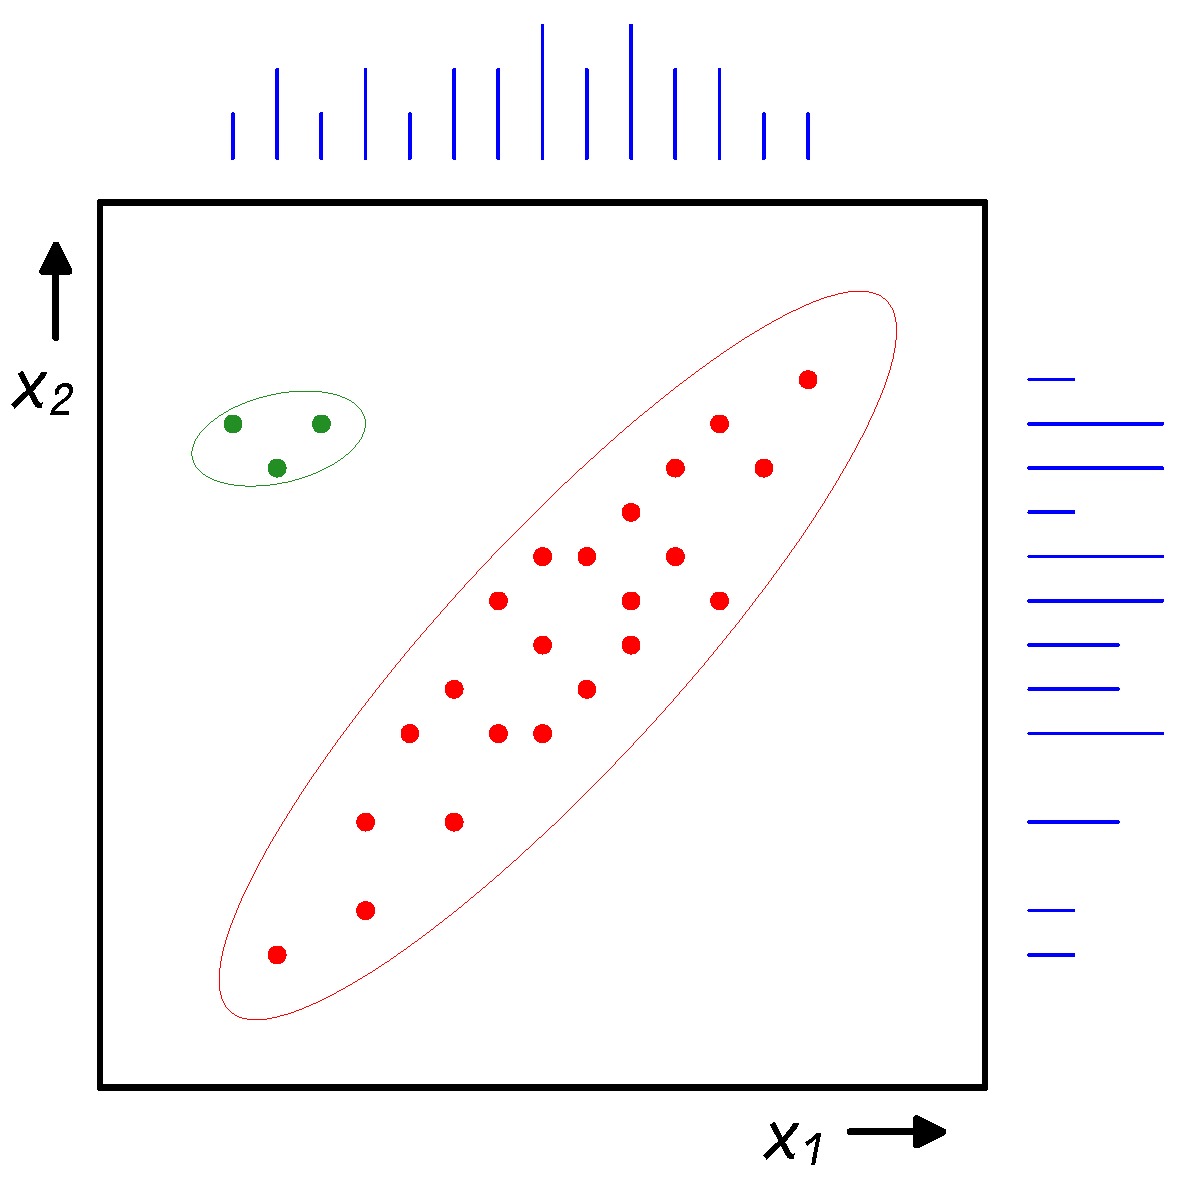
\includegraphics[width=0.75\textwidth]{Graphics/MultivariateNormal}
\end{figure}

Another problem occurs if the data distribution is not multivariate normal. For example, if the data really contain two distinct populations, the centroid calculated will be located between the populations and have no meaning (see fig. \ref{fig:MultNorm}). Of course, \arr{S} would also be meaningless. Methods to detect violation of multivariate normality are discussed in section \ref{text:MulNorm} on page \pageref{text:MulNorm}.

\subsubsection{The multivariate median}

\begin{figure}
 \caption{Two-dimensional example of convex hull stripping. The outermost data are iteratively removed, until only the data of the innermost hull remain, here a single data point. The centroid of this innermost hull is the multivariate median. For details see text.}
 \label{fig:Hull}
 \centering
 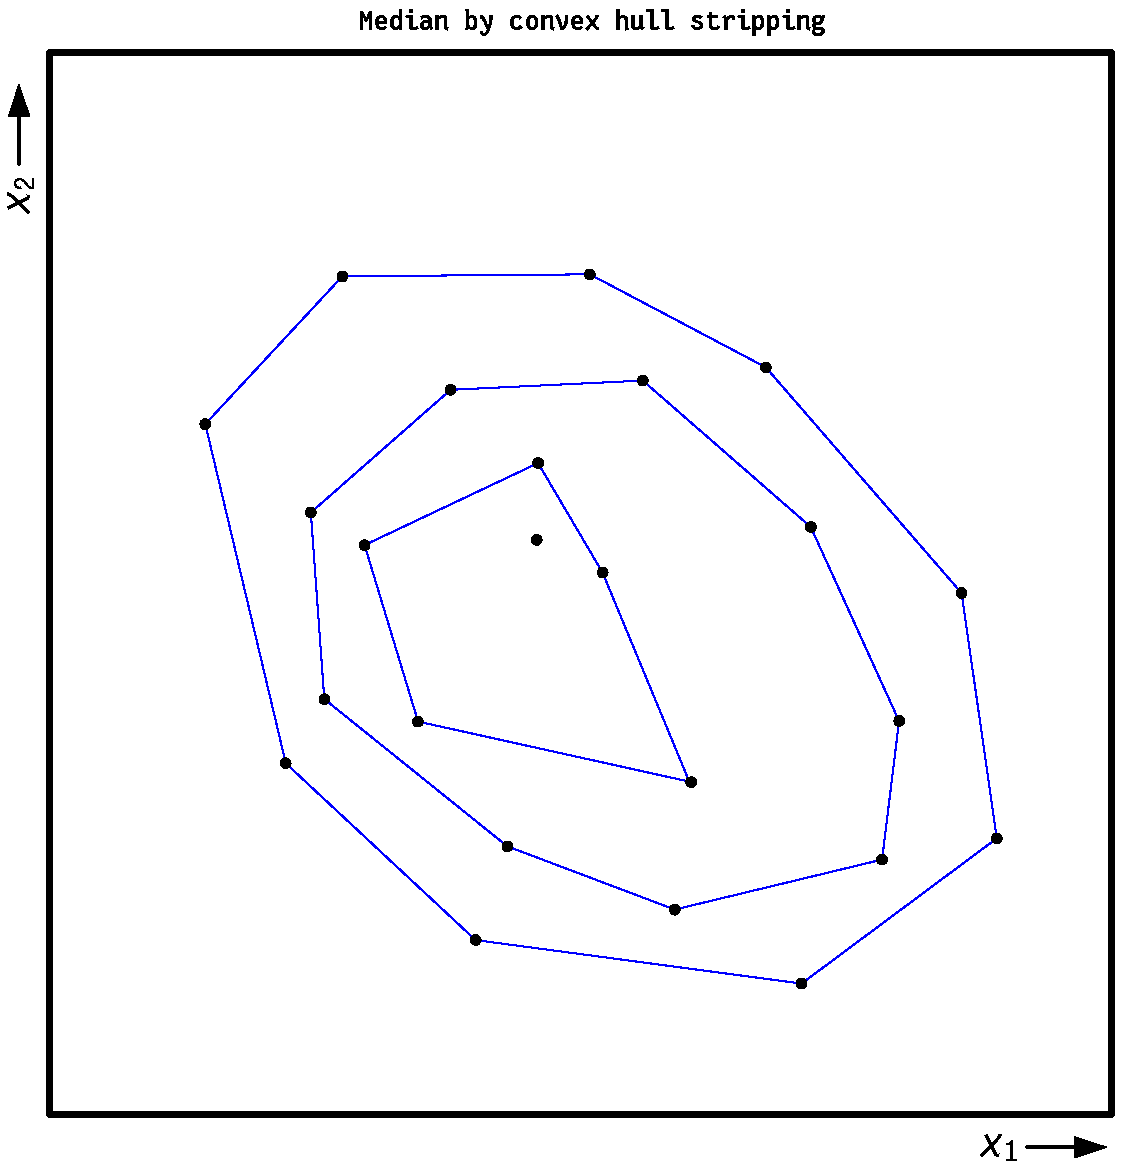
\includegraphics[width=0.75\textwidth]{Graphics/HullStripping}
\end{figure}


A data vector can be sorted, and hence its median determined. For a matrix, this is not possible. Several definitions of the multivariate median are used \parencite{Sma-90}, of which the conceptually most useful are:
\begin{description}
  \item[vector of medians]{is appropriate only if the variables in the data set are orthogonal (uncorrelated, say, after \acs{PCA}). }
  \item[\skalar{\ell 1} Median]{is the point of the data cloud that minimises the sum of the distance to all data points \( \sum_{i=1}^n{||\AbsVec{x}_i - \hat{\mu}||} \) (position of warehouse that optimally supplies all customers). It has a breakdown-point of \SI{50}{\%} and reduces to the standard median in the 1D-case. Unfortunately, there is no efficient algorithm for finding it.}
  \item[convex hull stripping]{For calculation of the univariate median, we recursively remove the largest and smallest values, until we are left with either one value (which is the median) or two (then the median is in between). This idea can be extended to multiple dimensions, by finding the hull of the data cloud. The hull is a convex polygon that encloses all data points with maximal area and minimal circumference. These points are removed, the new hull is calculated and removed and so on, until all remaining points are on the innermost hull. If this innermost hull consists of a single point, this point is the median, otherwise, the centroid is used (see fig. \ref{fig:Hull}).
      However, the breakdown point is \skalar{1/n} under unfavourable circumstances (if all data are on the hull). The median is also not a continuous function of the data in the matrix \arr{X}. }
  \item[Simplicial depth median]{If, in the 1D case, we construct all possible pairs of data points, then the median is the point which is enclosed by the largest number of these intervals, it is \emph{deep inside} the data cloud. This can be extended to \skalar{p} dimensions by replacing the intervals with simplexes \skalar{S(\AbsVec{x}_1, \ldots \AbsVec{x}_{p+1})}. Then
      \begin{equation}
        \mathrm{SDF}(\mu) = \binom{n}{p+1}^{-1} \sum_{1\leq i_1< \ldots < i_{p+1} \leq n}{1[\mu \in S(\AbsVec{x}_1, \ldots \AbsVec{x}_{p+1})]}
      \end{equation}
      Then the simplicial depth median is the point \skalar{\hat{\mu}}, that maximises SDF(\skalar{\mu}).
      }
\end{description}

\section{Test program}

\begin{lstlisting}
  PROGRAM TestDescript;

  USES math, MathFunc, Vector, Matrix, Zufall, Deskript;

  CONST ProbSize = 100;
        Vars     =   2;

  VAR Data, Weights, Dm, Dr       : VectorTyp;
      i, j                        : WORD;
      MinEle, MaxEle, sum, mean,
      std, q1, q2, q3, e2, e3, e4 : float;
      MData, DataWithWeights      : MatrixTyp;

  BEGIN
    CreateVector(Data, ProbSize, 0.0);
    CreateVector(Weights, ProbSize, 1/ProbSize);
    FOR i := 1 TO ProbSize DO
      SetVectorElement(Data, i, 100 + RandomNormal(0, 10));

    Mean := ArithmeticMean(Data);
    Writeln('Arithmetic mean: ', FloatStr(Mean, 10));
    Writeln('Geometric mean: ', FloatStr(GeometricMean(Data), 10));
    Writeln('Harmonic mean: ', FloatStr(HarmonicMean(Data), 10));
    Writeln;
    Writeln('Power mean, k=1: ', FloatStr(GeneralMean(Data, Weights, 1), 10));
    Writeln('Power mean, k=0.001: ', FloatStr(GeneralMean(Data, Weights, 0.001), 10));
    Writeln('Power mean, k=-1: ', FloatStr(GeneralMean(Data, Weights, -1), 10));
    Writeln;
    std := StandardDeviation(Data);
    Writeln('Standard deviation', FloatStr(std, 10));
    Writeln('excess kurtosis', FloatStr(ExcessKurtosis(Data, mean, std), 10));
    Writeln('Skewness', FloatStr(Skewness(Data, mean, std), 10));
    Writeln;
    Writeln('Gini coefficient: ', FloatStr(Gini(Data, Mean), 10));
    Writeln('Herfindahl-Index: ', FloatStr(HerfindahlIndex(Data), 10));
    Writeln;
    q2 := Median(Data);
    q1 := Quantile(Data, 0.25);
    q3 := Quantile(Data, 0.75);
    Writeln('Median: ', FloatStr(q2, 10));
    Writeln('Trimedian: ', FloatStr(Trimedian(Data), 10)); // data have been sorted by Median
    Writeln('Inter-quartile distance: ', FloatStr(InterQuantilDistance(q1, q3), 10));
    Writeln('MAD: ', FloatStr(MAD(Data), 10));
    Writeln('std. error of median: ', FloatStr(StandardErrorOfMedian(Data), 10));
    Writeln;
    Writeln('Naive Hodges-Lehmann: ', FloatStr(NaiveHodgesLehmann(Data), 10),
    ' Hodges-Lehmann estimator: ', FloatStr(HodgesLehmann(Data), 10)); // data have been sorted by Median
    Writeln('Naive Sn: ', FloatStr(NaiveSn(Data), 10), ' Sn: ', FloatStr(Sn(Data), 10));
    Writeln('Naive Qn: ', FloatStr(NaiveQn(Data), 10));
  //  Writeln('Qn: ', FloatStr(Qn(Data), 10));

    FOR i := 1 TO ProbSize DO SetVectorElement(Weights, i, RandomNormal(1/ProbSize, 0.01));
    MaxEle := FindLargest(Weights);
    MinEle := FindSmallest(Weights);
    Scale(Weights, MinEle, MaxEle); // weights IN 0..1
    Sum := TotalSum(Weights);
    FOR i := 1 TO ProbSize DO
      SetVectorElement(Weights, i, GetVectorElement(Weights, i)/Sum); // total weight = 1
    CreateMatrix(DataWithWeights, ProbSize, 2, 0.0);
    SetColumn(DataWithWeights, Data, 1);
    SetColumn(DataWithWeights, Weights, 2);
    Writeln;
    Write('Weighted median: ', FloatStr(WeightedMedian(DataWithWeights), 10));
    Writeln(', weighted LoMed:  ', FloatStr(WeightedLoMed(DataWithWeights), 10),
            ', weighted HiMed:  ', FloatStr(WeightedHiMed(DataWithWeights), 10));
    Writeln;
    e2 := ell2(Data);
    e3 := ell3(Data);
    e4 := ell4(Data);
    Writeln('ell2: ', FloatStr(e2, 10), ', ell3: ', FloatStr(e3, 10), ', ell4: ', FloatStr(e4, 10));
    Writeln('tau2: ', FloatStr(e2/mean, 10), ', tau3: ', FloatStr(e3/e2, 10), ', tau4: ', FloatStr(e4/e2, 10));
    Writeln('Ouartile coefficient of skewness: ', FloatStr(QuartileCoefficientOfSkewness(q1, q2, q3), 10));
    Writeln('Centile coefficient of kurtosis: ', FloatStr(CentilCoeffKurtosis(Data), 10));
    ReadLn;
    DestroyVector(Data);
    DestroyMatrix(DataWithWeights);

    CreateMatrix(MData, ProbSize, Vars, 0.0);
    FOR i := 1 TO (ProbSize DIV 10) DO              // 10% outliers
      BEGIN
        SetMatrixElement(MData, i, 1, 115 + RandomNormal(0, 3));
        SetMatrixElement(MData, i, 2, 110 + RandomNormal(0, 3));
      END;
    FOR i := Succ(ProbSize DIV 10) TO ProbSize DO   // 90% inliers
      BEGIN
        SetMatrixElement(MData, i, 1, 110 + RandomNormal(0, 3));
        SetMatrixElement(MData, i, 2, 115 + RandomNormal(0, 3));
      END;
    RobustDistance (MData, Dr);
    MahalanobisDistance (MData, Dm);
    FOR i := 1 TO ProbSize DO
      Writeln(i:3, ' ', FloatStr(GetMatrixElement(MData, i, 1), 11), ' ',
      FloatStr(GetMatrixElement(MData, i, 2), 11), ' ',
      FloatStr(GetVectorElement(Dm, i), 10), ' ', FloatStr(GetVectorElement(Dr, i), 10));

    ReadLn;
    DestroyVector(Dr);
    DestroyVector(Dm);
    DestroyMatrix(MData);
  END.
\end{lstlisting}

\printbibliography[heading=subbibliography]
\end{refsection}
